\clearpage
\section{Well-posedness for spatially irregular ODEs}\label{chap:wellposed}

The main results of this chapter regard first-order, one-dimensional IVPs $x'=f(t,x)$, $x(\tau)=\xi$, where $f$ belongs to the subset $\uF\subset\uC(\RR^2,\RR)$ from \autoref{ch:intro}, repeated here for convenience.

\textbf{\autoref{def:driving_func}} (Set $\uF$ of functions)\textbf{.}
    Let the subset $\uF\subset\uC(\RR^2,\RR)$ contain the functions $f$ such that $f(\cdot,x)$ is strictly increasing for every $x\in\RR$, and $f(\tau,\xi)>0$ for some $(\tau,\xi)\in\RR^2$.

The focus of this chapter is well-posedness for these IVPs specifically, which for us means addressing questions related to the existence and uniqueness, continuous dependence and simulation of solutions. Following \cite{lipschitz_1876} and the extensive line of spatial regularity-based uniqueness theory, e.g.~collected tremendously in \cite{agarwal_1993}, the well-posedness of \emph{maximal} solutions for such IVPs, i.e.~well-posedness for \autoref{prob:ivp}, has not yet been considered. This is despite ODEs depending implicitly on such functions in $\uF$ appearing in Wolfgang Doeblin's 1940 treatment of diffusions (presented like \autoref{eq:tce} in a `time-changed' form), as discussed in \autoref{ch:intro} and extensively in \cite{bru_2002}.

Local uniqueness theory for IVPs driven by functions in $\uF$ does exist, and $f(\cdot,x)$ can be relaxed to being non-decreasing even. This line of research can be considered to originate from a simple uniqueness result in \cite{peano_1890}, but essentially terminates with \cite{wend_1969}. This is covered in more detail in \autoref{sec:uniqueness}. The most relevant consequence of this terminal article is presented as Theorem 2.6.1 in \cite{agarwal_1993}, but is omitted from mainstream texts like the classic \cite{hartman_2002}. The practical problem is \emph{precisely} this locality, which reduces the time interval $[\tau,T)$ of consideration until we know $f(t,\vp(t))>0$ holds for a local solution $\vp\in\uC^1([\tau,T),\RR)$. Given this, a uniqueness proof becomes straightforward, and is accommodated by the general work of \cite{cid_2009}.

The impracticality of this locality constraint was discussed in \autoref{ch:intro} alongside an IVP deriving from the Heston model in \autoref{eq:heston_intro}, which is important in volatility modelling. Considering \autoref{eq:hest_ode}, fix $\sigma,\kappa,\theta,v>0$ and $w\in\uC_0(\RR,\RR)$, then define $f\in\uF$ using
\begin{equation}\label{eq:cir_ivp_well_posed}
    f(t,x) := \sigma w(x) + \kappa(\theta t - x) + v.
\end{equation}
Then although, for each $w\in\uC_0(\RR,\RR)$, existing theory provides the uniqueness of a local solution $\vp$ to the IVP $x'=f(t,x)$, $x(0)=0$ over some interval $[0,T)$, it is still possible (in fact probable, in volatility modelling) that there is no fixed interval over which this theory can be applied almost surely, when $w$ is drawn under Brownian motion's Wiener measure.

So no fixed interval $[0,T)$ exists over which a coherent volatility model can be defined using existing ODE theory, even in this relatively simple Heston example in \autoref{eq:cir_ivp_well_posed}. This clarifies a shortcoming of local results like \cite{wend_1969} and \cite{cid_2009} for probabilistic applications, helping to explain why these are not in the mainstream theory. With this in mind, new results here include statements like the following immediate consequence of \autoref{thm:global_uniqueness}, which does not prohibit finding $\vp'(t)=f(t,\vp(t))=0$ for some $t>\tau$.

\begin{corollary}[Maximal uniqueness]\label{thm:uniqueness_toy}
    Provided $f\in\uF$ and $f(\tau,\xi)>0$, the IVP $x'=f(t,x)$, $x(\tau)=\xi$ has a unique maximal solution. This is to say, \autoref{prob:ivp} has a unique solution.
\end{corollary}

Recall from \autoref{ch:intro} that solutions $\vp$ of such IVPs will model paths of a price process's cumulative variance, with corresponding volatility $\sqrt{\vp'}$. So we are not interested in initial values $(\tau,\xi)\in\RR^2$ where $\vp'(\tau)=f(\tau,\xi)<0$. As in \autoref{thm:uniqueness_toy} above, this chapter further assumes $f(\tau,\xi)>0$, because treating the case of $f(\tau,\xi)=0$ is delicate. This treatment is reserved until \autoref{sec:refining_problem}, where we look closer at the solution set of such IVPs, and confirm that this accommodates all strictly increasing and differentiable paths. The consequences of this for volatility paths $\sqrt{\vp'}$ are deceptively rich. For example, while it is quite clear that $\vp'$ cannot be zero over intervals, \cite{royden_2010} use pathological examples to show $\vp'$ can still be zero on a set of points arbitrarily close to full Lebesgue measure.

We will shortly provide an `additively separable' class of IVP examples in \autoref{sec:main_problem} which are relevant to the entirety of this thesis, but for now we demonstrate one specific example of the familiar Heston case in \autoref{eq:cir_ivp_well_posed}, to build intuition for the diverse functions in $\uF$.

In \autoref{eq:cir_ivp_well_posed} we have the freedom to fix any $w\in\uC_0(\RR,\RR)$, so can choose Karl Weierstrass's pathological function, studied notably in \cite{hardy_1916}, with its H\"older regularity properties established in \cite{zygmund_2003}. This admits the Fourier series representation
\begin{equation}\label{eq:weierstrass_def}
    w(x) := \sum_{k\in\NN_0}a^{-\alpha k}\sin(2 a^k\pi x).
\end{equation}
For any $\alpha\in(0,1)$, this series converges provided $a$ is an odd integer greater than 5, by the Weierstrass M-test, and the path $w$ is then nowhere differentiable, but $\alpha$-H\"older continuous. This is demonstrated in \autoref{fig:weierstrass_example}, alongside a corresponding function $f$ from \autoref{eq:cir_ivp_well_posed}. The blue arrows in the right panel, like in the related figures which will follow, provide the direction of the vector $(1,f(t,x))$, to which ODE solutions are necessarily tangential. Notice how the points where $f(t,x)=1$ form a graph over the $x$ axis, which is clearly related to $w$.

\begin{figure}[ht]
    \centering
    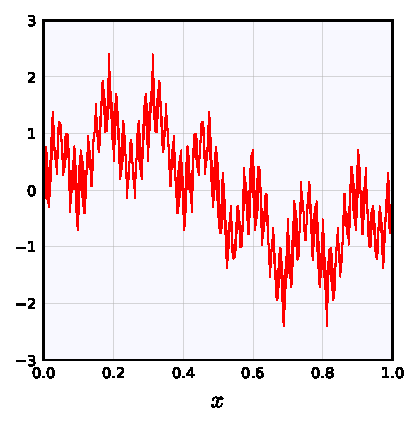
\includegraphics[height=0.48\linewidth]{figures/weierstrass1}
    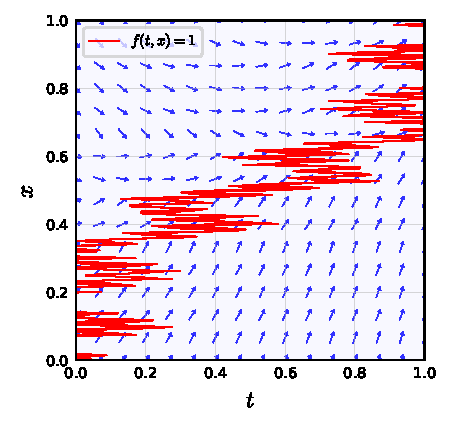
\includegraphics[height=0.48\linewidth]{figures/weierstrass2}
    \caption{The left panel shows the Weierstrass path $w$ from \autoref{eq:weierstrass_def}, with $a=7$ and $\alpha=0.25$. The right panel demonstrates the corresponding Heston function $f$ (blue arrows) from \autoref{eq:cir_ivp_well_posed}, with $\sigma=0.25$, $\kappa=2$ and $v=\theta=1$. Also shown is the path where $f(t,x)=f(0,0)=1$.}
    \label{fig:weierstrass_example}
\end{figure}

Once uniqueness for such highly irregular IVPs is in place, practically relevant properties of the wider modelling framework fall into place. For example, define the truncated functions
\begin{equation}\label{eq:truncated_weierstrass}
    w_n(x):=\sum_{k=0}^n a^{-\alpha k}\sin(2a^k\pi x),\quad f_n(t,x) := \sigma w_n(x) + \kappa(\theta t - x) + v,
\end{equation}
for $n\in\NN$, which unlike $w$ or $f$ can be stored exactly in computer memory. Then, the continuous dependence result of \autoref{thm:continuity_solution_map} establishes that the solutions $\vp_n$ of the IVPs $x'=f_n(t,x)$, $x(0)=0$ will converge to the unique solution of the IVP $x'=f(t,x)$, $x(0)=0$ uniformly over compacts as $n\to\infty$, and the simulation convergence result of \autoref{thm:euler_converge} similarly establishes the convergence of computationally friendly forward Euler polygons.

\vspace{2mm}
Now moving on, the present chapter is structured as follows. \autoref{sec:main_problem} precisely defines the class of spatially irregular IVPs being treated in this chapter, and provides example subsets $\uF_\vt\subset\uF$ of functions containing all of the Heston-related ones referred to thus far. \autoref{sec:function_zeros} takes a step back, analysing the zeros of any function $f\in\uF$. Although not directly related to IVPs, this cannot not be neglected, being important for many of the results which follow. \autoref{sec:global_bijectivity} treats the maximal existence of IVP solutions, but also establishes some basic properties of solutions, like them being strictly increasing, important for volatility modelling. \autoref{sec:uniqueness}, \autoref{sec:cont_dep} and \autoref{sec:simulation} then focus specifically on the uniqueness, continuous dependence and simulation of maximal solutions respectively.

\subsection{The main problem and examples}\label{sec:main_problem}

The programme of this section is to first reiterate the class of IVPs discussed in \autoref{ch:intro} depending on the set $\uF\subset\uC(\RR^2,\RR)$ of functions, to which the main results in this chapter will apply, and to then provide simple subsets $\uF_\vt\subset\uF$ of examples which accommodate the IVPs mentioned thus far, e.g.~those deriving from the Heston case in \autoref{eq:cir_ivp_well_posed}.

Recall that it is \autoref{prob:ivp} to which this chapter applies, repeated here for convenience.

\textbf{\autoref{prob:ivp}} (IVPs of \autoref{chap:wellposed})\textbf{.}
    For $f\in \uF$ and $(\tau,\xi)\in\RR^2$ where $f(\tau,\xi)>0$, find a maximal solution $\vp\in\uC^1([\tau,T_*),\RR)$ of the IVP $x'=f(t,x)$, $x(\tau)=\xi$. By definition, this means $\vp$ verifies $\vp'(t)=f(t,\vp(t))$ for each $t\in[\tau,T_*)$, $\vp(\tau)=\xi$ and also $T_*\vee\sup_{t\in[\tau,T_*)}|\vp(t)|=\infty$.

Some minor points are in order. Firstly, through the statement of \autoref{prob:ivp} it is clear we are only seeking solutions $\vp$ defined over some set $[\tau,T_*)$, i.e.~extending \emph{forwards} in time from initial conditions $(\tau,\xi)$. As discussed in \autoref{ch:intro}, `histories' extending backwards in time will be considered in \autoref{chap:solutions}. As such we should interpret $\vp'(\tau)$ as a right derivative.

Recall that should we find a solution $\vp$ in a set $\uC^1([\tau,T_*),\RR)$ for some $T_*\in(\tau,\infty]$, then it is only the condition $T_*\vee\sup_{t\in[\tau,T_*)}|\vp(t)|=\infty$ which distinguishes this as a \emph{maximal} solution. This condition means $\vp$ must extend to the boundary of $\RR^2$, i.e.~as far as possible. For $\vp$ to be such a solution, thereby verifying $\vp'(t)=f(t,\vp(t))$ over $[\tau,T_*)$ and $\vp(\tau)=\xi$, is equivalent to $\vp$ verifying the integral equation $\vp(t)=\xi+\int_\tau^t f(s,\vp(s))\dd s$. Although this requires proof, this can be found in any ODE text, e.g.~p.2 of \cite{coddington_1955}.

Finally, as in the title of this thesis, we refer to the IVP in \autoref{prob:ivp} as `spatially irregular', because we have not imposed regularity conditions, such as Lipschitz or H\"older continuity, on the spatial component of the functions in $\uF$. `Temporally strictly increasing and spatially irregular' certainly provides a more complete description. But, loosely, although our IVPs being strictly increasing in their temporal variable renders them \emph{helpful} for volatility modelling, i.e.~ensures that volatility $\sqrt{\vp'}$ is well-defined given a solution $\vp$, it is the spatial irregularity of these IVPs which thereafter governs \emph{how helpful}, via the IVPs' solution set, and distinguishes the resulting modelling framework from comparatively restrictive others.

For example, due to this irregularity, the solution set becomes so large that, unlike in the conventional framework depending on It\^o SDEs, the highly irregular paths of volatility observed in reality, with very low, time-varying, or even no apparent  H\"older regularity, can be accommodated. See \cite{bennedsen_2022} for extensive empirical evidence of such volatility paths, and the recent research into `hyper' or `super' rough volatility models, such as \cite{jusselin_2020} and \cite{bayer_2021}. Hence our emphasis on a `spatially irregular' description, given our focus on volatility modelling.

We now look at some examples of \autoref{prob:ivp}, in which the functions in $\uF$ admit the additively separable representation $f(t,x)=\vt(t)-w(x)$ for some $\vt,w\in\uC(\RR,\RR)$. These examples may seem related to the work of \cite{kaper_1988} at first, wherein the authors consider similarly separable functions. But the assumptions there are actually very different, e.g.~$w$ is assumed monotone and differentiable except at the IVP starting point.

\begin{example}[The subsets $\uF_\vt\subset\uF$]\label{ex:main_example}
    Let the path $\vt\in\uC_0(\RR,\RR)$ be strictly increasing and bijective, so $\lim_{t\to\pm\infty}\vt(t)=\pm\infty$, then let the set $\uF_\vt$ contain functions with representation
    \begin{equation}\label{eq:main_example}
        f(t,x) := \vt(t) - w(x)
    \end{equation}
    for some $w\in\uC(\RR,\RR)$ with $w(0)<0$ and $\sup_{x\in\RR_+}w(x)=\infty$. For any such $\vt$, the inclusion $\uF_\vt\subset\uF\subset\uC(\RR^2,\RR)$ is then quite clear using \autoref{def:driving_func}, given that each $f(\cdot,x)$ is strictly increasing. Moreover, given that $f(0,0)>0$ is ensured, then for any $f\in\uF_\vt$ the IVP $x'=f(t,x)$, $x(0)=0$ provides an example of \autoref{prob:ivp}, specifically with $(\tau,\xi)=(0,0)$.
\end{example}

The assumptions related to $\infty$ in \autoref{ex:main_example} can be ignored for now, but are tremendously helpful later. We will specifically use the assumption  $\sup_{x\in\RR_+}w(x)=\infty$ (which is e.g.~satisfied almost surely by paths of Brownian motion) to guarantee maximal solutions of IVPs $x'=f(t,x)$, $x(0)=0$ are always global, i.e.~remain finite over all of $\RR_+$, for example. The unnecessary minus sign used in \autoref{eq:main_example} will be justified later as well, in \autoref{ex:zeros_example}.

Letting $\Theta$ contain the functions $\vt$ in \autoref{ex:main_example}, then to see that we \emph{do not} have the set equivalence $\cup_{\vt\in\Theta}\uF_\vt=\uF$ we can consider functions of type $f(t,x) = \vt_1(\vt_2(t) - w(x))$, where $\vt_{1,2}\in\Theta$, and also of multiplicative type $f(t,x) = \vt(t)w(x)$ provided $w$ is strictly positive. We will not explore such functions in our applications because we have no reason to believe they would be more helpful for volatility modelling than those in $\uF_\vt$. Notice the Heston function in \autoref{eq:cir_ivp_well_posed} is found in $\uF_\vt$ with $\vt(t):=\kappa\theta t$, provided $\sup_{x\in\RR_+}\kappa x - \sigma w(x)=\infty$.

\begin{figure}[H]
    \centering
    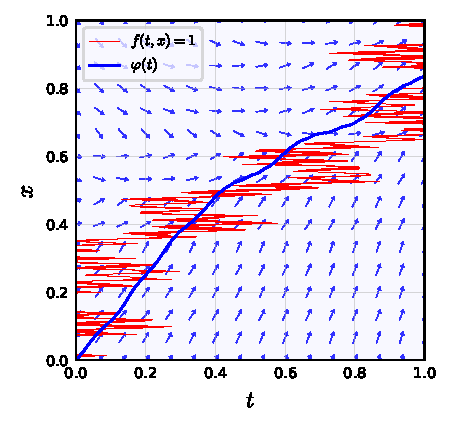
\includegraphics[height=0.48\linewidth]{figures/weierstrass3}
    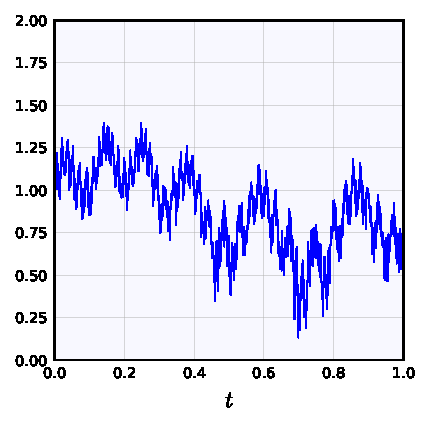
\includegraphics[height=0.48\linewidth]{figures/weierstrass4}
    \caption{The left panel repeats the right one in \autoref{fig:weierstrass_example} but includes the solution $\vp$ of the IVP $x'=f(t,x)$, $x(0)=0$. The right shows the corresponding `rough' volatility path $\sqrt{\vp'}$.}
    \label{fig:main_examples}
\end{figure}

\vspace{-4mm}
In \autoref{fig:main_examples} we illustrate a \emph{solution} $\vp$ of an IVP $x'=f(t,x)$, $x(0)=0$ where $f\in\uF_\vt$, using the Heston function from the right panel of \autoref{fig:weierstrass_example}, so $\vt(t):=\kappa\theta t$. Also shown in \autoref{fig:main_examples} is the corresponding volatility path $\sqrt{\vp'}$, which clearly inherits properties of the driving Weierstrass function from the left panel of \autoref{fig:weierstrass_example}. Of course both $\vp$ and $\vp'$ must be approximated using a simulation scheme, for which we use that from \autoref{alg:forward_euler}.

\begin{figure}[H]
    \centering
    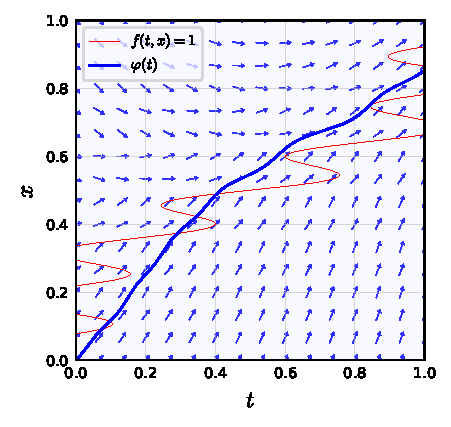
\includegraphics[height=0.48\linewidth]{figures/weierstrass3a}
    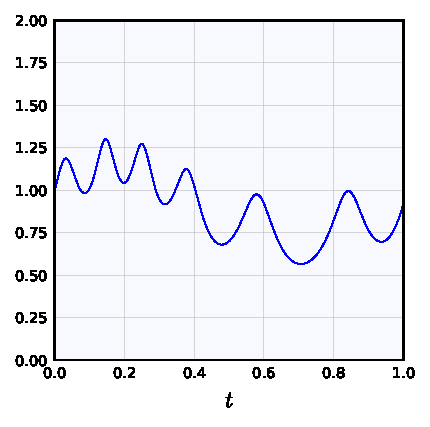
\includegraphics[height=0.48\linewidth]{figures/weierstrass4a}
    \caption{A reproduction of \autoref{fig:main_examples}, but using the truncated differentiable path $w_n$ from \autoref{eq:truncated_weierstrass} with $n=1$, rather than the $\alpha$-H\"older Weierstrass limit as $n\to\infty$.}
    \label{fig:main_examples2}
\end{figure}

\vspace{-3mm}

We now move on to consider the zeros of a function $f\in\uF$, i.e.~the points in $\RR^2$ where $f(t,x)=0$, which are related to the points where $f(t,x)=1$, as shown in \autoref{fig:main_examples}. Notice that for $f\in\uF_\vt$, these zeros verify the simple equation $\vt(t)=w(x)$, justifying the minus sign in \autoref{eq:main_example}. So these zeros also verify $t = \vt^{-1}(w(x))$, given $\vt\in\uC_0(\RR,\RR)$ is bijective.

\subsection{Driving functions' zeros}\label{sec:function_zeros}

For $f\in\uF$, understanding the points in $\RR^2$ where $f(t,x)=0$ turns out to be incredibly fruitful. For example, some basic properties of IVP solutions established in this chapter, the limit theorems of \autoref{chap:solutions} and the martingality result in \autoref{chap:framework} all depend on the c\`adl\`ag path $\bvp$ defined in \autoref{lem:zeros2} here, related to the path defined earlier in \autoref{eq:path_bound}. Because every $f(\cdot,x)$ is strictly increasing, these zero points can be characterised by a single path $\phi$, as covered in \autoref{lem:zeros1}. However, because it is also possible that no point $t\in\RR$ exists where $f(t,x)=0$ for a given $x\in\RR$, we choose to extend the image of $\phi$ beyond $\RR$.

So let $\bRR:=\RR\cup\{\pm\infty\}$ denote the extended real line, and $[x,\infty]:=[x,\infty)\cup\infty$ etc.~for $x\in\RR$. We equip $\bRR$ (and subintervals) with the standard topology (or `two-point compactification') which is homeomorphic, for example, to the Euclidean topology on $[-1,1]$. This can be induced by the metric $d(a,b):=|\tanh(b)-\tanh(a)|$ on $\bRR$, with $\tanh(\pm\infty):=\pm 1$, for example. \cite{aliprantis_1998} can be consulted for more details. Now denote by $\uC(\RR,\bRR)$ and $\uD(\RR,\bRR)$ the sets of paths which are respectively continuous and c\`adl\`ag given these topologies.

Adopt the conventions $\sup\varnothing:=-\infty$ and $\inf\varnothing:=\infty$. This enables the compact definition of $\phi\in\uC(\RR,\bRR)$ in \autoref{lem:zeros1}, although it is informative to check that this is equivalent to
\begin{equation}\label{eq:define_phi_alt}
\phi(x) :=
\begin{cases}
    -\infty & f(t,x)>0\ \forall t \\
    +\infty & f(t,x)<0\ \forall t \\
    t\in\RR \text{ such that } f(t,x)=0 & \text{otherwise}.
\end{cases}
\end{equation}
This next result \autoref{lem:zeros1} is related to the implicit function theorem e.g.~presented as in Theorem 9.28 of \cite{rudin_1976}, although we do not assume differentiability of $f$. Our proof relies upon the Bolzano-Weierstrass theorem for sequences (a bounded sequence in $\RR$ has a convergent subsequence), which is given as Theorem 3.4.8 in \cite{bartle_2011}.

\begin{lemma}[Path of zeros]\label{lem:zeros1}
    For $f\!\in\!\uF\!\subset\!\uC(\RR^2,\RR)$, define the function $\phi=\phi_f\!:\!\RR\to\bRR$ by
    \begin{equation}\label{eq:define_phi}
    \phi(x) := \sup\{t\in\RR: f(t,x) <0 \}.
    \end{equation}
    Then $\phi$ is a well-defined path in $\uC(\RR,\bRR)$, verifying $f(\phi(x),x)=0$ whenever $\phi(x)\in\RR$.
\end{lemma}
\begin{proof}
    It is clear, using \autoref{eq:define_phi}, that $\phi:\RR\to\bRR$ is a well-defined function, and the three cases in the representation of \autoref{eq:define_phi_alt} just follow from $\sup\varnothing:=-\infty$, $\sup\RR=\infty$ and the continuity of each strictly increasing $f(\cdot,x)$ respectively. Whenever $\phi(x)\in\RR$, then we are in the third case in \autoref{eq:define_phi_alt}, so clearly $f(\phi(x),x)=0$, and to establish the claim it just remains to show this function $\phi$ is in $\uC(\RR,\bRR)$. The proof here uses limits of sequences.

    So let $\{x_n\}_{n\in\NN_0}\subset\RR$ be a sequence with $x_n\xrightarrow{n\to\infty}x_0$ in $\RR$, but, for a contradiction, assume that $\phi(x_n)\xrightarrow{n\to\infty}\phi(x_0)$ is violated in $\bRR$. This divergence provides an open ball $\BB\subset\RR$ around $\phi(x_0)$ such that infinitely many $\phi(x_n)$ are in $\bRR\setminus\BB$. By considering a subsequence of $\{x_n\}_{n\in\NN_0}$ if necessary, we can therefore w.l.o.g.~assume that $\phi(x_n)\in\bRR\setminus\BB$ for every $n\in\NN_0$.

    Since the topology on $\bRR$ is homeomorphic to the Euclidean one on $[-1,1]$, the Bolzano-Weierstrass theorem provides a subsequence $\{x_{n_k}\}_{k\in\NN}$ verifying $\phi(x_{n_k})\xrightarrow{k\to\infty}t_0\in\bRR$. Importantly, $t_0\neq\phi(x_0)$ follows from having ensured $\phi(x_n)\in\bRR\setminus\BB$ for every $n$, opposing $\phi(x_0)\in\BB$. By again redefining $\{x_n\}_{n\in\NN_0}$ if necessary, we may assume w.l.o.g.~that $\phi(x_n)\xrightarrow{n\to\infty}t_0\neq\phi(x_0)$ holds. Now assume $t_0<\phi(x_0)$, and fix any $t_*\in(t_0,\phi(x_0))\subseteq\RR$.

    Using \autoref{eq:define_phi_alt}, if $\phi(x_0)=\infty$, then we have $f(t_*,x_0)<0$ by definition, and if $\phi(x_0)<\infty$, then $f(t_*,x_0)<f(\phi(x_0),x_0)=0$ follows from $f(\cdot,x_0)$ being strictly increasing. So $f(t_*,x_0)<0$ is ensured. Since $\phi(x_n)\xrightarrow{n\to\infty}t_0<t_*$, we can assume w.l.o.g.~that $\phi(x_n)<t_*$ for each $n$. Like previously, if $\phi(x_n)=-\infty$, then $f(t_*,x_n)>0$ by definition, and if $\phi(x_n)>-\infty$, then $0=f(\phi(x_n),x_n)<f(t_*,x_n)$ follows from each $f(\cdot,x_n)$ being strictly increasing. So $f(t_*,x_n)>0$ is ensured for each $n$. The continuity of $f$ now provides the contradiction
    \begin{equation}
        0<f(t_*,x_n)\xrightarrow{n\to\infty}f(t_*,x_0)<0.
    \end{equation}

    The analysis for $t_0>\phi(x_0)$ is practically identical, with these inequalities reversed. Due to these contradictions, the convergence $\phi(x_n)\xrightarrow{n\to\infty}t_0:=\phi(x_0)$ in $\bRR$ must hold. So, for any sequence $\{x_n\}_{n\in\NN_0}$, the convergence $x_n\xrightarrow{n\to\infty}x_0$ in $\RR$ implies $\phi(x_n)\xrightarrow{n\to\infty}\phi(x_0)$ in $\bRR$. This is equivalent to the outstanding claim of $\phi\in\uC(\RR,\bRR)$, so the proof is thus complete.
\end{proof}

The path $\phi\in\uC(\RR,\bRR)$ clearly \emph{characterises} the zeros of $f$, and an entire set $\{\phi_a\}_{a\in\RR}$ of paths could be similarly defined, where $f(\phi_a(x),x)=a$. The red line in \autoref{fig:main_examples} where $f(t,x)=1$ thus coincides with $\phi_1(x)$. With some work, using differential inequalities, each such path $\phi_a\in\uC(\RR,\bRR)$ can be used to construct a bound on any solution $\vp$ of the corresponding IVP $x'=f(t,x)$, $x(\tau)=\xi$. We will just focus on $\phi = \phi_0$, which specifically leads to the path $\bvp$ defined properly in \autoref{lem:zeros2}, which is established later as a solution bound in \autoref{lem:spatial_bounds}.

For $\phi\in\uC(\RR,\bRR)$ and $(\tau,\xi)\in\RR^2$, the next result \autoref{lem:zeros2} utilises `exit-time' notation $E(\phi) = E_{\tau,\xi}(\phi)$, which refers to the function defined over $[\tau,\infty)$, with $\inf\varnothing:=\infty$, through
\begin{equation}\label{eq:exit_def}
    E(\phi)(t) := \inf\{x>\xi:\phi(x)>t\}.
\end{equation}
The exit-time \emph{functional} $E$ is specified properly in \autoref{def:exit_functional}, but these details are superfluous now. It is however very helpful to note some properties of the function $E(\phi)$ defined in \autoref{eq:exit_def}, which are analysed extensively in Section 13.6 of \cite{whitt_2002}.

To this end, allow $\phi$ to be any path in $\uD(\RR,\RR)$ verifying $\sup_{x\in[\xi,\infty)}\phi(x)=\infty$. Then it is clear that $E(\phi)(\tau)\ge\xi$, and indeed $E(\phi)(t)\in[\xi,\infty)$ for each $t\in[\tau,\infty)$, given that $\sup_{x\in[\xi,\infty)}\phi(x)=\infty$. It is also clear that $E(\phi)$ is non-decreasing. Less clear is that $E(\phi)$ is c\`adl\`ag, so defines a path in $\uD([\tau,\infty),[\xi,\infty))$. Towards this, notice that left limits exist at any $t_*\in[\tau,\infty)$ since, over $[\tau,t_*)$, $E(\phi)$ is monotone and bounded in $[\xi,E(\phi)(t_*)]$. Similarly for right limits. Right continuity is best observed by contradiction: fixing any $x_*:=E(\phi)(t_*)$, then due to the use of `$\phi(x)>t$' in \autoref{eq:exit_def} (opposing `$\phi(x)\ge t$'), the inequality $\sup_{x\in[x_*,x_*+\ep)}\phi(x)>\phi(x_*)$ holds for every $\ep>0$. If a right discontinuity is assumed, namely a point $t_*\in[\tau,\infty)$ where $x_*^+:=\lim_{t\downarrow t_*}E(\phi)(t)>E(\phi)(t_*)=:x_*$, then $\sup_{x\in[x_*,x_*+\ep)}\phi(x)>\phi(x_*)$ is violated for every $\ep\in(0,x_*^+-x_*)$. Finally, there are two situations which can render $E(\phi)$ non-\emph{increasing} over an interval: either $\phi(\xi)>\tau$, then the interval is $[\tau,\phi(\xi))$, or given an upward discontinuity $\lim_{x\uparrow x_*}\phi(x)=:\phi(x_*^-)<\phi(x_*)$, then the interval is $[\phi(x_*^-),\phi(x_*))$. Assuming $\phi(\xi)\le\tau$ and $\phi\in\uC(\RR,\RR)$ therefore precludes such intervals, making $E(\phi)$ \emph{strictly} increasing. Continuous mapping properties of the related functional $E$ are also obtained in \cite{whitt_1971}, and exploited in \cite{puhalskii_1997}.

In what follows, minor extensions to these observations will be made, specifically to accommodate the two main differences here, following \autoref{lem:zeros1}, where $\phi$ is in $\uC(\RR,\bRR)$ rather than $\uC(\RR,\RR)$, and where $\sup_{x\in[\xi,\infty)}\phi(x)<\infty$ is possible rather than $\sup_{x\in[\xi,\infty)}\phi(x)=\infty$.

\begin{lemma}[C\`adl\`ag zeros]\label{lem:zeros2}
    Adopt the assumptions of \autoref{lem:zeros1}. Then for any initial value $(\tau,\xi)\in\RR^2$ where $f(\tau,\xi)\ge0$, define the function $\bvp=\bvp_{f,\tau,\xi}:[\tau,\infty)\to[\xi,\infty]$ by
    \begin{equation}\label{eq:up_bound}
        \bvp(t):=\inf\{x>\xi:f(t,x)<0\}.
    \end{equation}
    Then $\bvp$ is a well-defined increasing path in $\uD([\tau,\infty),[\xi,\infty])$, verifying $\bvp = E(\phi) = E_{\tau,\xi}(\phi)$. Moreover, if $\bvp(T)<\infty$, then $\bvp$ is \emph{strictly} increasing and verifies $f(t,\bvp(t))=0$ over $[\tau,T]$.
\end{lemma}
\begin{proof}
    Using \autoref{eq:up_bound}, for $t_*\in[\tau,\infty)$, either $\bvp(t_*)=\inf\varnothing:=\infty$ or, by the continuity of $f$, $\bvp(t_*)$ is the lowest value $x_*\in[\xi,\infty)$ where $f(t_*,x)<0$ for all $x$ in some $(x_*,x_*+\ep)$. This clarifies that $\bvp:[\tau,\infty)\to[\xi,\infty]$ is a well-defined function. If this lowest value $x_*=\bvp(t_*)<\infty$ indeed exists, then $f(t_*,x)\ge0$ for $x$ in $[\xi,x_*]$, while $f(t_*,x)<0$ for $x\in(x_*,x_*+\ep)$, so the continuity of $f$ also ensures $f(t_*,x_*)=f(t_*,\bvp(t_*))=0$. Since $\phi$ from \autoref{lem:zeros1} characterises the zeros of $f$, with $f(\phi(x),x)=0$ when $\phi(x)\in\RR$, then $t_* = \phi(x_*)\in\RR$.

    Now the equivalence $\bvp = E(\phi)$ will be established, meaning $\bvp(t)=\inf\{x>\xi:\phi(x)>t\}=:E(\phi)(t)$ over $[\tau,\infty)$. First assume $x_*=\bvp(t_*)<\infty$. If $\phi(x)<\infty$ for $x\in(x_*,x_*+\ep)$, then the ordering $f(t_*,x)<0=f(\phi(x),x)$ holds, and $t_*=\phi(x_*)<\phi(x)$ then follows from $f(\cdot,x)$ being strictly increasing. But clearly $\phi(x_*)<\phi(x)$ also holds if $\phi(x)=\infty$. Now assuming that $x_*\in[\xi,\infty)$ is \emph{not the lowest} value with $\phi(x)>\phi(x_*)$ for $x$ in some $(x_*,x_*+\ep)$, so \emph{not} equal to $E(\phi)(t_*)$, contradicts $x_*=\bvp(t_*)$ being the lowest value in $[\xi,\infty)$ where $f(t_*,x)<0$ for $x\in(x_*,x_*+\ep)$, again using that $f(\cdot,x)$ is strictly increasing. This establishes the equivalence $\bvp(t_*)=E(\phi)(t_*)$ for $t_*\in[\tau,\infty)$ \emph{when} $\bvp(t_*)<\infty$. If instead $\bvp(t_*)=\infty$, so $f(t_*,x)\ge0$ for $x\in[\xi,\infty)$, then $\phi(x)\le t_*$ holds over the same interval $[\xi,\infty)$, and $E(\phi)(t_*)=\infty$. This clarifies that $\bvp=E(\phi)$ holds whether $\infty$ is attained or not.

    It just remains to show that $\bvp=E(\phi)$ is in $\uD([\tau,\infty),[\xi,\infty])$ and is increasing or strictly increasing as claimed. The discussion following \autoref{eq:exit_def} clarifies that $E(\phi)$ is strictly increasing and in $\uD([\tau,\infty),[\xi,\infty))$ when $\phi\in\uC(\RR,\RR)$, $\phi(\xi)\le\tau$ and $\sup_{x\in[\xi,\infty)}\phi(x)=\infty$.

    In our case, $\phi(\xi)\le\tau$ clearly holds if $\phi(\xi)=-\infty$, and otherwise is ensured by $f(\phi(\xi),\xi)=0\le f(\tau,\xi)$ and $f(\cdot,\xi)$ being strictly increasing. The consequence of having $\phi\in\uC(\RR,\bRR)\supset\uC(\RR,\RR)$ is just that a point $x_*\in(\xi,\infty)$ could exist where $\lim_{x\uparrow x_*}\phi(x)=\infty$. But assuming $x_*$ to be the lowest such point, then $E(\phi)$ is clearly just found in $\uD([\tau,\infty),[\xi,x_*))$. Likewise, the effect of having $\sup_{x\in[\xi,\infty)}\phi(x)=t_*<\infty$ is simply that $E(\phi)(t)=\infty$ for all $t\in[t_*,\infty)$, using $\inf\varnothing:=\infty$, meaning now $E(\phi)$ is found in $\uD([\tau,\infty),[\xi,\infty])$. In all cases, $\bvp=E(\phi)$ remains in $\uD([\tau,\infty),[\xi,\infty])$, is strictly increasing over any $[\tau,T]\subset[\tau,\infty)$ provided $\bvp(T)<\infty$, and is constant over any $[T,\infty)\subset[\tau,\infty)$ if $\bvp(T)=\infty$, therefore the proof is complete.
\end{proof}

Showing that the path $\phi$ of zeros from \autoref{lem:zeros1} is in $\uC(\RR,\bRR)$ might seem superfluous, but this route appears to be the cleanest towards establishing properties of the path $\bvp$ in \autoref{lem:zeros2}, which are not at all obvious, yet critically important. As an example, if $\phi$ was only continuous into the weaker `one-point compactification' of $\RR$, so e.g.~could jump between $-\infty$ and $\infty$, then the resulting path $\bvp$ is not guaranteed to be strictly increasing.

For our volatility modelling applications, it would be acceptable to assume that any function $f\in\uF\subset\uC(\RR^2,\RR)$ is such that each $f(\cdot,x)$ defines a strictly increasing \emph{bijection} from and to $\RR$, like the Heston case in \autoref{eq:cir_ivp_well_posed} and all functions in the subsets $\uF_\vt\subset\uF$ from \autoref{ex:main_example}. In this case, it is straightforward to show that the zero path $\phi$ from \autoref{eq:define_phi} is in $\uC(\RR,\RR)$. Although tempting to make this bijectivity assumption, the extended reals $\bRR$ are still required to make sense of the more important c\`adl\`ag path $\bvp$ from \autoref{lem:zeros2}, unless $\bvp(t)<\infty$ can be ensured over $[\tau,\infty)$ by further constraints. So at least in this chapter, we stay in the general setting where $f$ simply belongs to $\uF$, and so $\phi\in\uC(\RR,\bRR)$.

The following example clarifies the forms of these two paths, $\phi\in\uC(\RR,\bRR)$ and $\bvp\in\uD(\RR_+,\bRR_+)$, when $f$ is in a subset $\uF_\vt\subset\uF$ from \autoref{ex:main_example}, and when $(\tau,\xi)=(0,0)$. For convenience, let the subsets $\Theta,\uW\subset\uC(\RR,\RR)$ contain the paths $\vt$ and $w$ from \autoref{ex:main_example} respectively.

\begin{example}[The subset $\uF_\vt\subset\uF$]\label{ex:zeros_example}
    Recall functions $f\in\uF_\vt$ admit the representation
    \begin{equation}
        f(t,x) := \vt(t) - w(x),
    \end{equation}
    where $(\vt,w)\in\Theta\times\uW$. Using \autoref{eq:define_phi}, the path $\phi$ from \autoref{lem:zeros1} is then given by
    \begin{equation}
        \phi(x) := \sup\{t\in\RR: f(t,x) <0 \} = \sup\{t\in\RR: \vt(t) < w(x) \} = \vt^{-1}(w(x)),
    \end{equation}
    where the final representation $\phi=\vt^{-1}\circ w$ follows from our assumption that $\vt\in\Theta$ is bijective. The path $\phi$ is thus found in $\uC(\RR,\RR)$, i.e.~we never find $\phi(x)=\pm\infty$, and have $f(\phi(x),x)=0$ for all $x\in\RR$. Now from \autoref{eq:up_bound}, the corresponding path $\bvp$ is given by
    \begin{equation}
        \bvp(t):= \inf\{x>0:f(t,x)<0\} = \inf\{x>0:w(x)>\vt(t)\}.
    \end{equation}
    Given that $w\in\uW$ ensures $\sup_{x\in\RR_+}w(x)=\infty$, then we find $\bvp(t)<\infty$ over $\RR_+$. Combining this with \autoref{lem:zeros2}, then $\bvp$ defines a strictly increasing path in $\uD(\RR_+,\RR_+)$ where $f(t,\bvp(t))=0$ holds, and finally we have the exit-time relationship $\bvp = E(\vt^{-1}\circ w)=E(\phi)$.
\end{example}

Following these examples, now specifically let $f$ take the Heston form in \autoref{eq:cir_ivp_well_posed}, so
\begin{equation}
    f(t,x) := \sigma w(x) + \kappa(\theta t - x) + v,
\end{equation}
which is found in $\uF_\vt$, with $\vt(t):=\kappa\theta t$, provided $\sup_{x\in\RR_+}\kappa x - \sigma w(x)=\infty$. Then we find
\begin{equation}\label{eq:zeros_example4}
    \phi(x) := (\kappa\theta)^{-1}(\kappa x - \sigma w(x) - v),\quad \bvp(t):=\inf\{x>0: \kappa x - \sigma w(x) > \kappa\theta t + v\}.
\end{equation}
The form of $\bvp$ coincides with that given in \autoref{eq:path_bound} which, as discussed in \autoref{ch:intro}, can be considered as a path of an IG L\'evy process. The left panel of \autoref{fig:function_zeros} demonstrates both paths from \autoref{eq:zeros_example4}, which should be compared with the left panel of \autoref{fig:main_examples}. To help visualise $\bvp$ (the discontinuities of which are technically dense) and the relationship $\bvp=E(\phi)$ of \autoref{lem:zeros2}, the intervals $\bvp_*(t):=[\bvp(t_-),\bvp(t)]$ are shown in the right panel.

\begin{figure}[H]
    \centering
    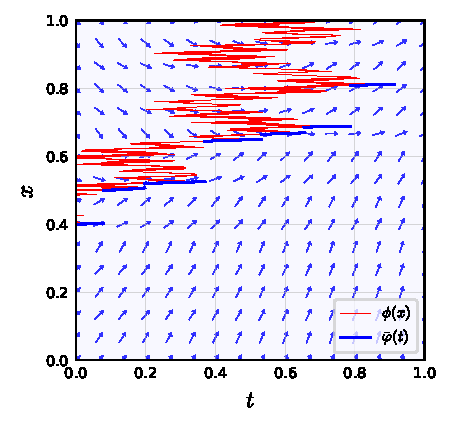
\includegraphics[height=0.46\linewidth]{figures/weierstrass6a}
    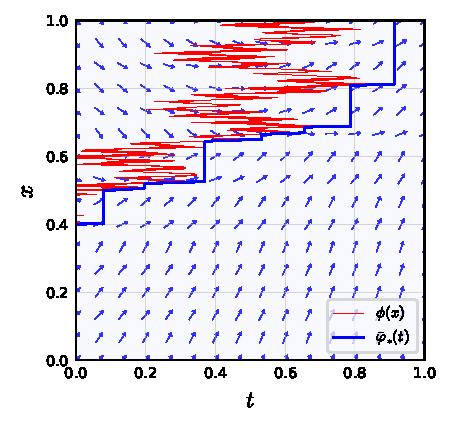
\includegraphics[height=0.46\linewidth]{figures/weierstrass6}
    \caption{The left panel shows the paths $\phi$ and $\bvp$ from \autoref{eq:zeros_example4}, where the Weierstrass path $w$ and parameters $\sigma,\kappa,\theta,v$ are consistent with those in \autoref{fig:main_examples}. The right panel repeats the left but shows instead $\bvp_*(t):=[\bvp(t_-),\bvp(t)]$.}
    \label{fig:function_zeros}
\end{figure}

\subsection{Maximal existence, bijectivity and bounds}\label{sec:global_bijectivity}

The focus henceforth is IVP solutions of \autoref{prob:ivp}, and not just properties of the driving functions $f\in\uF$, like in the previous section. Specifically, the main programme of this section is as follows. First, in \autoref{lem:spatial_bounds}, spatial bounds of solutions are established which, as stated in \autoref{thm:bijectivity_new}, help clarify that maximal solutions $\vp$ are bijective paths in some set $\uC^1([\tau,T_*),[\xi,X_*))$ with $T_*\vee X_*=\infty$. This was discussed following the statement of \autoref{prob:ivp}. \autoref{lem:temporal_unbound} and \autoref{lem:spatial_unbound} then provide simple conditions on $f$ which help control the values of $T_*\in(\tau,\infty]$ and $X_*\in(\xi,\infty]$ respectively, so e.g.~$T_*=X_*=\infty$ can be ensured. As discussed before \autoref{def:mod_driving_func}, this is desirable for volatility modelling. Finally, following \autoref{ex:main_example}, consequences of these results are given in the example of $f\in\uF_\vt$.

\vspace{3mm}\textbf{Solution bounds.} Considering simple geometrical consequences of the next result, as demonstrated in \autoref{fig:function_zeros}, it becomes clear that the spatial solution bounds $\xi\le\vp(t)\le\bvp(t)$ established restrict solutions into a subsets of $[\tau,\infty)\times[\xi,\infty)$ where $f(t,x)\ge0$, leading to the desired strictly increasing solutions. It is important to appreciate that this does \emph{not} mean that the region where instead $f(t,x)<0$ can be neglected, or replaced arbitrarily. On the contrary, this region is required to define the important path $\bvp$ from \autoref{lem:zeros2}.

Proof of \autoref{lem:spatial_bounds} here utilises differential inequalities, as covered extensively in \cite{lakshmikantham_1969}. Full details are provided here, however, given that we make unconventional use of such inequalities over \emph{c\`adl\`ag} paths related to $\bvp\in\uD([\tau,\infty),[\xi,\infty])$.

Use of such paths makes this result more complicated that it can seem, and making use of the path $\phi\in\uC(\RR,\bRR)$ from \autoref{lem:zeros1} and mean value theorem (MVT), rather than directly using $\bvp$, can seem superfluous. This is because, although \autoref{eq:spatial_bound} provides $f(t,x)<0$ for $x$ in some interval $(\bvp(t),\bvp(t)+\ep)$, the infimum of such $\ep$ values over any time interval will be zero if the discontinuities of $\bvp$ are dense in $[\tau,T_*)$. This is the situation a.s.~in the Heston example of \autoref{eq:zeros_example4}, so is practically relevant, and means we cannot make use of a set of paths $\bvp_\ep(t):=\bvp(t)+\ep$ above $\bvp$ where $f(t,\bvp_\ep(t))<0$, which would simplify matters.

\begin{lemma}[Spatial solution bounds]\label{lem:spatial_bounds}
    Assume $f\in\uF$ and $f(\tau,\xi)>0$, then define $\bvp$ by
    \begin{equation}\label{eq:spatial_bound}
        \bvp(t) := \inf\{x>\xi:f(t,x)<0\},
    \end{equation}
   which adheres to \autoref{lem:zeros2}. Then any maximal solution $\vp$ of the IVP $x'=f(t,x)$, $x(\tau)=\xi$, which is in some set $\uC^1([\tau,T_*),\RR)$ with $T_*\in(\tau,\infty]$, satisfies $\xi\le\vp(t)\le\bvp(t)$ over $[\tau,T_*)$.
\end{lemma}
\begin{proof}
    The lower bound of $\xi\le\vp(t)$ is simple to establish. Because $\vp'(\tau) = f(\tau,\xi) > 0$, then $\vp(t)>\xi$ is ensured for all $t$ in some $(\tau,\tau+\ep)$, and so $\vp$ enters the quadrant $(\tau,\infty)\times(\xi,\infty)$. A first touching point $t_*>\tau$ where $\vp(t_*)=\xi$ then provides $\vp'(t_*)\le0$, given $\vp(t)$ must approach $\xi$ from above. But $f(\cdot,\xi)$ is strictly increasing, so we run into the contradiction
    \begin{equation}
        0 \ge \vp'(t_*) = f(t_*,\vp(t_*)) = f(t_*,\xi) > f(\tau,\xi) >0,
    \end{equation}
    and instead must conclude that $\vp(t)>\xi$ for all $t\in(\tau,T_*)$. Establishing the upper bound of $\bvp$ is conceptually similar, but complicated by the fact that $f(t,\bvp(t))=0$ whenever $\bvp(t)<\infty$, as shown in \autoref{lem:zeros2}, rather than the more helpful $f(t,\bvp(t))<0$. Moreover, as noted before this result, trying to utilise values $\ep>0$ such that $f(t,x)<0$ for all $x\in(\bvp(t),\bvp(t)+\ep)$ is futile, since the infimum of such $\ep$ values is zero over any interval where $\bvp$ jumps. So we make use of the path $\phi\in\uC(\RR,\bRR)$ of zeros from \autoref{lem:zeros1}, related to $\bvp$ through $\bvp=E(\phi)$.

    Since $f(\tau,\xi)>0$, it is clear from \autoref{eq:spatial_bound} and the continuity of $f$ that $\bvp(\tau)>\xi=\vp(\tau)$, so $\bvp$ is a strict bound at this starting point. Likewise, if for $t_*\in[\tau,T_*)$ we find $\bvp(t_*)=\infty$, then clearly the strict bound $\vp(t)<\bvp(t)=\infty$ also holds over $[t_*,T_*)$. The proof is thus trivially complete if $t_*=\tau$, which applies to impractical cases (for us) like $f(t,x):=1 + t$.

    Despite $\bvp$ being only c\`adl\`ag, if ever a point where $\vp(t)>\bvp(t)$ is found, a crossing point $t_*<t$ where $\vp(t_*)=\bvp(t_*)=:x_*$ is guaranteed, given $\vp(\tau)<\bvp(\tau)$ and $\bvp$ is strictly increasing. Assume a \emph{first} such crossing point $t_*\in(\tau,T_*)$ exists. Then given the relationship $\bvp=E(\phi)$, $\phi\in\uC(\RR,\bRR)$ \emph{and} that $t_*$ is the first crossing point, there exists $\ep,\delta>0$ such that the parametric path $(t,\vp(t))$ for $t\in(t_*,t_\delta)$ resides \emph{strictly} earlier in time than that of $(\phi(x),x)$ for $x\in(x_*,x_\ep)$, where $t_\delta:=t_*+\delta$ and $\vp(t_\delta)=x_\ep:=x_*+\ep$. For additional clarity, residing `strictly earlier in time' means $\vp(t)=x\implies t<\phi(x)$ whenever $(t,x)\in(t_*,t_\delta)\times(x_*,x_\ep)$.

    Given $\phi$ characterises the zeros of $f$ according to $f(\phi(x),x)=0$ by \autoref{lem:zeros1}, and every $f(\cdot,x)$ is strictly increasing, then having $(t,\vp(t))$ positioned earlier in time than $(\phi(x),x)$ provides $f(t,\vp(t))<0$ for $t\in(t_*,t_\delta)$. However, the MVT provides a point $t\in(t_*,t_\delta)$ where $\vp'(t)=(x_\ep-x_*)/(t_\delta-t_*)=\ep/\delta>0$. We have thus established  $f(t,\vp(t))<0<\vp'(t)$ at this point, and $\vp$ therefore cannot solve the ODE $x'=f(t,x)$ over $(t_*,t_\delta)\subset[\tau,T_*)$, if $t_*$ exists.

    The assumption of such a point in $[\tau,T_*)$ where $\bvp(t)<\vp(t)$ is therefore absurd, and $\vp(t)\le\bvp(t)$ thus extends from the initial time $\tau$ to the entirety of $[\tau,T_*)$, completing the proof.
\end{proof}

In the above proof, we saw that the bound of $\vp(t)\ge\xi$ is strict for all $t>\tau$, and with the geometry of this proof in mind it is worth covering conditions which make the upper bound $\vp(t)\le\bvp(t)$ also strict, over $[\tau,T_*)$. Towards this, assume that $\bvp$ is not \emph{just} strictly increasing, but verifies $\bvp(t)-\bvp(s)\ge\ep(t-s)$ for some $\ep>0$ and all $s,t\in[\tau,T_*)$ with $s\le t$. Now, if a first touching time $t_*\in(\tau,T_*)$ where $\vp(t_*)=\bvp(t_*)$ is assumed, then $\vp'(t_*)=0$, given $f(t_*,\bvp(t_*))=0$, but $\bvp(t)-\bvp(t_*)\le-\ep(t_*-t)<0$ for $t\in(\tau,t_*)$. So, a contradictory interval in $(\tau,t_*)$ is found where $\bvp(t)<\vp(t)$. Given the relationship $\bvp=E(\phi)$ from \autoref{lem:zeros2}, where $\phi\in\uC(\RR,\bRR)$ and $f(\phi(x),x)=0$ whenever $\phi(x)\in\RR$, then this property of $\bvp(t)-\bvp(t_*)\le-\ep(t_*-t)<0$ is ensured (by elementary geometrical considerations) given the \emph{one-sided} Lipschitz condition $\phi(x) - \phi(u) \le L (x - u)$ of \autoref{lem:strict_upper}, where $\ep:=L^{-1}$. One-sided Lipschitz properties can be found in \cite{lakshmikantham_1969} and \cite{agarwal_1993}, regarding bounds and uniqueness of solutions respectively.

\begin{lemma}[Strict upper bound]\label{lem:strict_upper}
    The upper bound in \autoref{lem:spatial_bounds} is strict, i.e. $\vp(t)<\bvp(t)$ over $[\tau,T_*)$, and $\vp'(t)>0$, if the path $\phi\in\uC(\RR,\bRR)$ from \autoref{lem:zeros1} has the one-sided Lipschitz property $\phi(x) - \phi(u) \le L (x - u)$ for some $L\in\RR_+$ and all $u,x\in[\xi,\infty)$ with $x\ge u$.
\end{lemma}

This result is practically relevant because a solution $\vp$, modelling the cumulative variance of a price path, then has a \emph{strictly} positive corresponding volatility $\sqrt{\vp'}$. This can be helpful, in order to relate abstract risk-neutral derivative pricing measures to a real-world probability measure (both introduced in \autoref{sec:martingale}), although the details of this will not be covered.

\vspace{3mm}\textbf{Bijective maximal solutions.} The main purpose of the bounds in \autoref{lem:spatial_bounds} for now is to help enable the bijectivity statement in the following result. The reader should note that the assumption $f(\tau,\xi)>0$ here cannot in general be relaxed to $f(\tau,\xi)\ge0$, which is treated in \autoref{sec:refining_problem}. Now recall, following the statement of \autoref{prob:ivp}, that a \emph{maximal} solution $\vp\in\uC^1([\tau,T_*),\RR)$ is one which reaches the boundary of $\RR^2$, i.e.~which verifies $T_*\vee\sup_{t\in[\tau,T_*)}|\vp(t)|=\infty$, and classical ODE theory, e.g.~Theorem 1.1.3 of \cite{lakshmikantham_1969}, establishes the existence of such solutions in our setting where $f\in\uC(\RR^2,\RR)$.

\begin{theorem}[Maximal existence and bijectivity]\label{thm:bijectivity_new}
    Assume $f\in\uF$ and $f(\tau,\xi)>0$. Then there exists a maximal solution $\vp$ of the IVP $x'=f(t,x)$, $x(\tau)=\xi$. Moreover, any such $\vp$ defines a strictly increasing bijection in some set $\uC^1([\tau,T_*),[\xi,X_*))$, where $T_*\vee X_*=\infty$.
\end{theorem}
\begin{proof}
    Classical theory gives the existence statement, since $f\in\uC(\RR^2,\RR)$. This provides a maximal solution $\vp\in\uC^1([\tau,T_*),\RR)$ which, by definition, satisfies $T_*\vee\sup_{[\tau,T_*)}|\vp(t)|=\infty$. Because $f\in\uF$ and $f(\tau,\xi)>0$, the bounds $\xi\le\vp(t)\le\bvp(t)$ hold over $[\tau,T_*)$ by \autoref{lem:spatial_bounds}.

    Given that $f(t,\xi)>f(\tau,\xi)>0$ for $t>\tau$, it is clear then from the definition $\bvp(t) := \inf\{x>\xi:f(t,x)<0\}$ that $\vp$ is restricted to a subset of $\RR^2$ where $f(t,x)\ge0$, making $\vp$ non-decreasing. Recall from \autoref{lem:zeros2} that $f(t,\bvp(t))=0$ when $\bvp(t)<\infty$, so a touching point $\vp(t)=\bvp(t)$ provides $\vp'(t)=0$. In the opposite direction, if $\vp'(t)=0$, then we must find either $\vp(t)=\bvp(t)$ or $\vp(t)=\bvp(t_-)<\bvp(t)$, given $\bvp$ is strictly increasing. So now, for a contradiction, assume $\vp'(t)=0$ holds over an interval $[a,b]\subset[\tau,T_*)$. Then we must find
    \begin{equation}
        \bvp(a_-)\le\bvp(a) = \vp(a) = \vp(b) = \bvp(b_-) \le \bvp(b).
    \end{equation}
    But having $\bvp(a)=\bvp(b_-)$ implies that $\bvp$ is constant at least over $[a,b)$, which violates the strictly increasing nature of $\bvp$ from \autoref{lem:zeros2}. So $\vp$ is non-decreasing, and $\vp'(t)=0$ \emph{cannot} hold over intervals. So in any such $[a,b]$ we must find a point where $\vp'(t)>0$, and the continuity of $\vp'$ extends this to ensure that $\vp(b)-\vp(a)=\int_a^b\vp'(s)\dd s>0$ for $a,b\in[\tau,T_*)$.

    Therefore, like $\bvp$, we find $\vp\in\uC^1([\tau,T_*),\RR)$ to be strictly increasing, and $\vp$ therefore defines a bijection in $\uC^1([\tau,T_*),[\xi,X_*))$, where $X_*=\lim_{t\uparrow T_*}\vp(t)\in(\xi,\infty]$. This allows the maximality condition $T_*\vee\sup_{[\tau,T_*)}|\vp(t)|=\infty$ to be written as $T_*\vee|\xi|\vee X_*=\infty$. In turn this is equivalent to the claim of $T_*\vee X_*=\infty$, given we know $|\xi|<\infty$, completing the proof.
\end{proof}

\vspace{3mm}\textbf{Existence conditions.} From the condition $T_*\vee X_*=\infty$ in \autoref{thm:bijectivity_new}, we know that either $T_*=\infty$, or $X_*=\infty$, or both. The purpose of the next two results is to provide separate practicable conditions on $f$ which independently ensure $T_*=\infty$ or $X_*=\infty$ respectively, both of which are desirable. Establishing the first of these is quite straightforward, as follows.

\begin{lemma}[Temporal existence]\label{lem:temporal_unbound}
    Let $f,\tau,\xi,\bvp$ be as defined in \autoref{lem:spatial_bounds}, and $\vp\in\uC^1([\tau,T_*),[\xi,X_*))$ be any maximal solution  of the IVP $x'=f(t,x)$, $x(\tau)=\xi$. If $\bvp(T)<\infty$ for some $T\in(\tau,\infty)$, then $T_*>T$, and by extension, if $\bvp(t)<\infty$ over $[\tau,\infty)$, then $T_*=\infty$.
\end{lemma}
\begin{proof}
    From \autoref{thm:bijectivity_new}, $\vp$ is a bijective element of some $\uC^1([\tau,T_*),[\xi,X_*))$ with $T_*\vee X_*=\infty$. For a contradiction, assume $\bvp(T)<\infty$ for some $T\in(\tau,\infty)$ but $T_*\le T<\infty$. Then we have $X_*=\infty$, so that $T_*\vee X_*=\infty$ is verified, and therefore $\vp(t)\xrightarrow{t\to T_*}\infty$. Because $\vp$ is strictly increasing over $[\tau,T_*)$ and $\bvp$ is over $[\tau,T]\supset[\tau,T_*)$, then having $\vp(\tau)=\xi<\bvp(\tau)$ and $\bvp(T)<\lim_{t\uparrow T_*}\vp(t)=\infty$ provides a unique touching point $t_*\in(\tau,T_*)$ where $\vp(t_*)=\bvp(T)$, with the strict inequalities $\bvp(t)<\bvp(T)<\vp(t)$ over $(t_*,T_*)$. This contradicts the relationship $\vp(t)\le\bvp(t)$ over $[\tau,T_*)$ from \autoref{lem:spatial_bounds}. So instead we find $T_*>T$ if $\bvp(T)<\infty$. The extension to $T_*=\infty$ follows this argument when letting $T\to\infty$, establishing the claim.
\end{proof}

The simple condition of $\bvp(T)<\infty$ in \autoref{lem:temporal_unbound} of course only ensures existence of maximal solutions over $[\tau,T]$ when $f\in\uF$, and not more generally when $f\in\uC(\RR^2,\RR)$. Nevertheless this is a condition which supplements classical existence theory, such as the main result of \cite{wintner_1945}, presented concisely as Theorem 5.1 in \cite{hartman_2002}. This theorem requires checking a limit $\int^\infty\dd x/U(t,x)=\infty$, for some $U$ with $|f(t,x)|\le U(t,|x|)$ over $[\tau,T]$, and applies to cases like $U(t,x)=x$ and $U(t,x)=x\log x$. But this condition depends on $f$ in an unbounded set like $[\tau,T]\times\RR$, so taking an example like $f(t,x):=t-w(x)$ with $w(x):=x^a\sin(x) - 1$ and any $a>1$, we find $\int^\infty\dd x/U(t,x)<\infty$ when making the natural selection $U(t,x)=1+t+x^a$, yet \autoref{lem:temporal_unbound} immediately provides existence of all maximal solutions over $[\tau,\infty)$, given that the upper bound $\bvp$ is the element of $\uD(\RR_+,\RR)$ given by
\begin{equation}\label{eq:exit_use1}
    \bvp(t) = \inf\{x>0: x^a\sin(x)-1>t\} = E(w)(t) < \infty.
\end{equation}

On the other hand, consider the reduction of this example to $f(t,x):=1 + t$, i.e.~using instead $w(x)=-1$. Then clearly $\vp(t):=t + \frac12 t^2$ is the global solution of $x'=f(t,x)$, $x(0)=0$. However, since one finds $\bvp(t):=\inf\{x>0:-1>t\}=\inf\varnothing:=\infty$ for all $t\in\RR_+$, \autoref{lem:temporal_unbound} is useless in this elementary example. But, as discussed after \autoref{def:solutionset}, such examples with $\liminf_{t\to\infty}\vp'(t)=\infty$ are not helpful when $\sqrt{\vp'}$ will model a volatility path.

Now we want a condition on $f\in\uF$ which can ensure $X_*=\infty$ in \autoref{thm:bijectivity_new}. Towards this, consider the example of $f(t,x):=2-e^{-t}-2x$. Then it is straightforward to check that $f\in\uF$ and  $\vp(t):=1-e^{-t}$ is a global solution of the IVP $x'=f(t,x)$, $x(0)=0$. In \autoref{thm:bijectivity_new} we therefore have $(T_*,X_*)=(\infty,1)$, i.e.~$\vp\in\uC^1(\RR_+,[0,1))$. The property of this IVP leading to $X_*=1<\infty$ is that $f(t,1)=-e^{-t}<0$ for all $t\in\RR_+$, so $\vp$ cannot pass through the line where $x=1$. Indeed, this is equivalent to having $\lim_{x\uparrow 1}\phi(x)=\infty$ where $\phi\in\uC(\RR,\bRR)$ is from \autoref{lem:zeros1}. The condition in the following result serves to rule out such examples, thereby enforcing $X_*=\infty$, in fact characterising this property when $f\in\uF$.

In the following statement, note that any such maximal solution $\vp$ is a bijective element of some set $\uC^1([\tau,T_*),[\xi,X_*))$ with $T_*\vee X_*=\infty$ by \autoref{thm:bijectivity_new}, so e.g.~$\vp(t)\xrightarrow{t\to T_*}X_*$ holds.

\begin{lemma}[Spatial existence]\label{lem:spatial_unbound}
    Assume $f\in\uF$ and $f(\tau,\xi)>0$. Then any maximal solution $\vp\in\uC^1([\tau,T_*),[\xi,X_*))$ of the IVP $x'=f(t,x)$, $x(\tau)=\xi$ satisfies $X_*>X$ iff $\lim_{t\to\infty}f(t,x)>0$ for all $x\in[\xi,X]$. So $X_*=\infty$ iff $\lim_{t\to\infty}f(t,x)>0$ for all $x\in[\xi,\infty)$.
\end{lemma}
\begin{proof}
    The easier only if direction is dealt with first, so suppose $X_*>X$ for some $X>\xi$. Given that $\vp\in\uC^1([\tau,T_*),[\xi,X_*))$ is bijective by \autoref{thm:bijectivity_new}, then $\vp(t)\xrightarrow{t\to T_*}X_*>X$ and there exists unique $T\in(\tau,T_*)$ where $\vp(T)=X$, with $\vp'(t)\ge0$ over $[\tau,T]$. So we find $f(t,\vp(t))= \vp'(t)\ge0$ over $[\tau,T]$, and given $\{\vp(t):t\in[\tau,T]\}=[\xi,X]$ and $f(\cdot,x)$ is strictly increasing, then clearly $\lim_{t\to\infty}f(t,x)>0$ for every $x\in[\xi,X]$. If $X_*=\infty$, this argument applies to any $X\in(\xi,\infty)$, so $\lim_{t\to\infty}f(t,x)>0$ for $x\in[\xi,\infty)$, completing half of the proof.

    In the other direction, we are trying to establish $X_*>X$ for some $X>\xi$. Notice that if $T_*<\infty$, then we must have $X_*=\infty>X$ to verify the requirement $T_*\vee X_*=\infty$ from \autoref{thm:bijectivity_new}. The result is thus obvious, and we should now assume $T_*=\infty$. Further suppose that for some $X\in(\xi,\infty)$, $\lim_{t\to\infty}f(t,x)>0$ holds for every $x\in[\xi,X]$. A time $T\in(\tau,T_*)$ will now be constructed where $\vp(T)>X$ must hold, confirming $X_*>X$. First notice that this condition of $\lim_{t\to\infty}f(t,x)>0$ implies $\phi(x)<\infty$ for $x\in[\xi,X]$, where $\phi$ from \autoref{lem:zeros1} characterises the zeros of $f$ according to $f(\phi(x),x)=0$ when $\phi(x)\in\RR$.

    For $\ep>0$, define the shifted path $\phi_\ep\in\uC([\xi,X],\RR)$ by $\phi_\ep(x):=(\tau\vee \phi(x))+\ep$. Then the strict inequality $f(\phi_\ep(x),x)>0$ holds, given every $f(\cdot,x)$ is strictly increasing. Now define
    \begin{equation}
        c:=\min_{x\in[\xi,X]} f(\phi_\ep(x),x)\in(0,\infty),\quad t_*:= \max_{x\in[\xi,X]}\phi_\ep(x) \in (\tau,\infty).
    \end{equation}
    These values ensure the inequality $f(t,x)\ge c$ on the vertical line $(t_*,x)$ for $x\in[\xi,X]$, so also $f(t,x)> c$ in the rectangle $(t_*,\infty)\times[\xi,X]$. Now define the time $T:=t_* + c^{-1}(X-\xi)$ and the line $\underline{\vp}\in\uC([t_*,T],[\xi,X])$, from points $(t_*,\xi)$ to $(T,X)$ with gradient $c>0$, by
    \begin{equation}
        \underline{\vp}(t):= \xi + c(t - t_*).
    \end{equation}
    We have constructed a line $\underline\vp$ where clearly $\underline\vp'(t)=c$, and also $f(t,\underline{\vp}(t))>c$ over $(t_*,T)$. Clearly $\ubvp(t_*)=\xi<\vp(t_*)$ holds, and assuming a first touching point where $\vp(t)=\ubvp(t)$, thus $\vp'(t)\le c$, provides the contradiction $c<f(t,\ubvp(t))=f(t,\vp(t))=\vp'(t)\le c$. So instead we must have $\vp(t)>\underline\vp(t)$ over $[t_*,T]$, and so also $\vp(T)>\underline\vp(T)=X$, confirming that $X_*>X$. By taking $X\to\infty$, the extension to $X_*=\infty$ is straightforward, completing the proof.
\end{proof}

The proof of \autoref{lem:spatial_unbound} is constructive in that it actually establishes a lower bound $\ubvp$ for the point $T\in(\tau,T_*)$, i.e.~verifying $\xi<\ubvp(T)<\vp(T)\le\bvp(T)$, so improves on the lower bound from \autoref{lem:spatial_bounds}. Such bounds, and their derivation via differential inequalities, are central to establishing the limit theorems of \autoref{chap:solutions}, especially \autoref{thm:exit_limit}, where it is natural to interpreted these \emph{not} as lower bounds in space, but rather upper bounds in time.

This next result just bring together those of \autoref{lem:temporal_unbound} and \autoref{lem:spatial_unbound}, in the way that these will be applied when treating \autoref{prob:ivp2} in \autoref{chap:solutions}. For this we present the condition $\bvp(t)<\infty$ from \autoref{lem:temporal_unbound} directly on $f\in\uF$ as $\inf_{x\in[\xi,\infty)}f(t,x)<0$, which is clearly equivalent using \autoref{eq:up_bound}. Similarly, the condition $\lim_{t\to\infty}f(t,x)>0$ of \autoref{lem:spatial_unbound} is presented as $\sup_{t\in[\tau,\infty)}f(t,x)>0$, which is equivalent given $f(\cdot,x)$ is strictly increasing. After the statement of \autoref{cor:exist_summary}, the purpose of the assumptions made in \autoref{eq:assumptions_G}, defining the subset $\uG\subset\uC(\RR^2_+,\RR)$ to which \autoref{chap:solutions} applies, will be clear.

Like for \autoref{lem:spatial_unbound}, by writing $\vp\in\uC^1([\tau,T_*),[\xi,X_*))$ in the following statement we mean the values $T_*,X_*$ are as established in \autoref{thm:bijectivity_new}, so e.g.~the limit $\vp(t)\xrightarrow{t\to T_*}X_*$ holds.

\begin{corollary}[Spatio-temporal existence]\label{cor:exist_summary}
    Assume $f\in\uF$ and $f(\tau,\xi)>0$. Then maximal solutions $\vp\in\uC^1([\tau,T_*),[\xi,X_*))$ of the IVP $x'\!=\!f(t,x)$, $x(\tau)\!=\!\xi$ verify the conditions~
    \begin{equation}\label{eq:exist_summary}
        \inf_{x\in[\xi,\infty)}f(t,x)<0\ \ \forall t\in[\tau,\infty)\implies T_*=\infty,\ \sup_{t\in[\tau,\infty)}f(t,x)>0\ \ \forall x\in[\xi,\infty)\implies X_*=\infty.
    \end{equation}
\end{corollary}

\vspace{2mm}This completes coverage of some basic properties of these spatially irregular IVPs from \autoref{prob:ivp}, and their solutions, and these properties are now clarified with examples depending on the subsets $\uF_\vt\subset\uF$ used in \autoref{ex:zeros_example}. Particularly notable is how the existence condition of $\inf_{x\in[\xi,\infty)}f(t,x)<0$ in \autoref{eq:exist_summary} places no constraint on the positive growth of $f(t,x)$ for $x\in[\xi,\infty)$, which  in \autoref{ex:global_exist} below is controlled by the negative growth of the paths $w\in\uW$. So the conditions of \autoref{eq:exist_summary} indeed supplement classical existence conditions depending on such positive growth constraints, as discussed following \autoref{lem:temporal_unbound}.

\begin{example}[The subset $\uF_\vt\subset\uF$]\label{ex:global_exist}
    Recall functions $f\in\uF_\vt$ admit the representation
    \begin{equation}
        f(t,x) := \vt(t) - w(x),
    \end{equation}
    where $(\vt,w)\in\Theta\times\uW$, so e.g.~$\lim_{t\to\pm\infty}\vt(t)=\pm\infty$ and $\sup_{x\in\RR_+}w(x)=\infty$. In \autoref{ex:zeros_example} we saw that the path $\bvp$ from \autoref{lem:zeros1} for the IVP $x'=f(t,x)$, $x(0)=0$ is then given by
    \begin{equation}
        \bvp(t)= \inf\{x>0:w(x)>\vt(t)\},
    \end{equation}
    and this is in $\uD(\RR_+,\RR_+)$, given $\sup_{x\in\RR_+}w(x)=\infty$. We can more compactly write this as $\bvp=E(\vt^{-1}\circ w)=E(w)\circ\vt$, using the exit-time notation from \autoref{eq:exit_def}. Now \autoref{thm:bijectivity_new} tells us that any maximal solution $\vp$ of this IVP is a bijective path in some set $\uC^1([0,T_*),[0,X_*))$, where $T_*\vee X_*=\infty$. Given $\bvp(t)<\infty$ for all $t\in\RR_+$, then \autoref{lem:temporal_unbound} provides $T_*=\infty$, and given $\lim_{t\to\infty}f(t,x)=\infty$ for every $x\in\RR$, then \autoref{lem:spatial_unbound} provides $X_*=\infty$ also. \autoref{cor:exist_summary} can equivalently be used to obtain $T_*=X_*=\infty$, that is
    \begin{equation}
        \inf_{x\in\RR_+}\vt(t) - w(x)<0\ \ \forall t\in\RR_+\implies T_*=\infty,\ \sup_{t\in\RR_+}\vt(t) - w(x)>0\ \ \forall x\in\RR_+\implies X_*=\infty.
    \end{equation}
\end{example}

\vspace{4mm}Following this example, now specifically let $f$ take the Heston form in \autoref{eq:cir_ivp_well_posed}, so
\begin{equation}
    f(t,x) := \sigma w(x) + \kappa(\theta t - x) + v,
\end{equation}
which is found in $\uF_\vt$, with $\vt(t):=\kappa\theta t$, provided $\sup_{x\in\RR_+}\kappa x - \sigma w(x)=\infty$. Then we have
\begin{equation}
    \bvp(t):=\inf\{x>0: \kappa x - \sigma w(x) > \kappa\theta t + v\}
\end{equation}
which, given $\sup_{x\in\RR_+}\kappa x - \sigma w(x)=\infty$, defines a path in $\uD(\RR_+,\RR_+)$ and provides an upper bound to any maximal solution $\vp$ of the IVP $x'=f(t,x)$, $x(0)=0$. Such maximal solutions are thus found in $\uC^1_0(\RR_+,\RR_+)$, as we hope when modelling volatility. In \autoref{fig:global_exist_examples} we illustrate solutions $\vp$ and their bounds $\bvp$ in this Heston setting, consistently with earlier figures.

\begin{figure}[H]
    \centering
    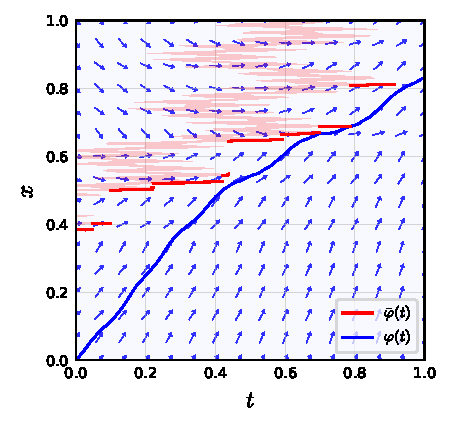
\includegraphics[height=0.46\linewidth]{figures/weierstrass7a}
    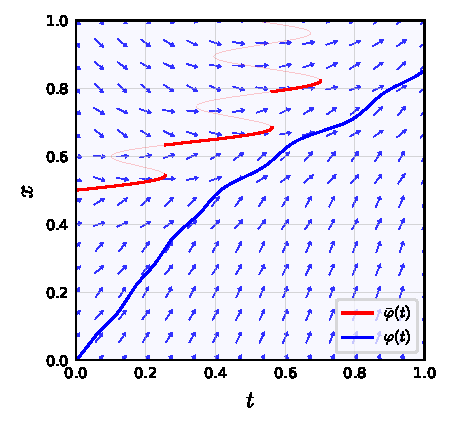
\includegraphics[height=0.46\linewidth]{figures/weierstrass7}
    \caption{Solutions $\vp$ of the IVP $x'=f(t,x)$, $x(0)=0$ are shown alongside their upper bounds $\bvp$ from \autoref{lem:spatial_bounds}. The functions $f$ are consistent with \autoref{fig:main_examples} and \autoref{fig:main_examples2}.}
    \label{fig:global_exist_examples}
\end{figure}

\subsection{Maximal uniqueness}\label{sec:uniqueness}

As promised at the beginning of this chapter, this section starts by clarifying what existing ODE uniqueness theory has to say about \autoref{prob:ivp}. An excellent starting point is the text \cite{agarwal_1993}, which systematically presents 21 directly applicable first-order ODE uniqueness theorems, as well as further corollaries, nonuniqueness theorems and `Carath\'eodory' extensions, which assume only the a.e.~differentiability of solutions.

\vspace{3mm}\textbf{Historical context.} The only existing result which places no constraints on the spatial behaviour of $f\in\uC(\RR^2,\RR)$, so could in principle be applied to \autoref{prob:ivp}, is that of \cite{wend_1969}, stated as Theorem 2.6.1 in \cite{agarwal_1993}. Technically, this is not quite true, since, for example, Theorem 1.21.2 due to \cite{yosie_1925}, which is the only which actually \emph{characterises} uniqueness, of course accommodates Wend's and all others. Although this characterisation is achieved very intuitively, with the result being so general it is hard to imagine establishing its conditions without having to use those of another.

Perhaps unsurprisingly, the situation in Wend's theorem is similar to ours, as covered in \autoref{ch:intro} when discussing the importance of maximal solutions. Specifically, a temporal monotonicity constraint is assumed, and solutions are sought only forwards in time. This result will be introduced properly shortly, but we first consider the earlier result of \cite{peano_1890}. This instead adopts a \emph{spatial} monotonicity constraint, and applies to examples like $f(t,x)=-\mathrm{sgn}(x)|x|^a$ for $a\in(0,1)$, which generate unique solution $\vp(t)=0$ through $(0,0)$.

\begin{theorem}[Peano's uniqueness]
    Let $f\in\uC(\RR^2,\RR)$ be such that $f(t,\cdot)$ is non-increasing for every $t\in\RR$. Then the IVP $x'=f(t,x)$, $x(\tau)=\xi$ has a unique maximal solution.
\end{theorem}

Proving this result takes just a few lines, and these are presented following Theorem 1.3.1 in \cite{agarwal_1993}. Now a consequence of the inverse function theorem, e.g.~Theorem 9.24 in \cite{rudin_1976}, is that if $\vp$ is a solution of an IVP $x'=f(t,x)$, $x(\tau)=\xi$ with a well-defined and differentiable inverse $\vp^{-1}$, then this inverse will solve the inverted IVP $x'=g(t,x)$, $x(\xi)=\tau$ where $g(t,x):=1/f(x,t)$. This is covered and utilised in \cite{cid_2009}. For now notice that the non-increasing assumption of $f(t,\cdot)$ from Peano's theorem becomes a non-\emph{decreasing} assumption on $g(\cdot,x)$, inverting the constraint between time and space and placing us in the setting which Wend's theorem applies. But also notice that since points where $f(x,t)=\infty$ are precluded in Peano's theorem by the assumption $f\in\uC(\RR^2,\RR)$, then we must preclude points where $g(t,x)=0$ manually in Wend's theorem.

\begin{theorem}[Wend's uniqueness]\label{thm:wend_uniqueness}
    Assume $f\in\uC(\RR^2,\RR)$, $f(\cdot,x)$ is non-decreasing for $x\in\RR$ and $f(t,x)>0$ in $\cX\subset\RR^2$ with $(\tau,\xi)\in\cX$. Then the IVP $x'=f(t,x)$, $x(\tau)=\xi$ has a unique solution in $\cX$, i.e.~some $\vp\in\uC^1([\tau,T],\RR)$ with $(t,\vp(t))\in\cX$ and $(T,\vp(T))\in\partial\cX$.
\end{theorem}

So Wend's theorem is a local result and not applicable to maximal solutions, unless the assumption of $f(t,x)>0$ in $\cX$ is extended to all of $\RR^2$. This is clearly not acceptable for volatility modelling, ruling out the Heston case at the core of this thesis, in \autoref{eq:cir_ivp_well_posed}, and generally rendering the important path $\bvp$ from \autoref{lem:zeros2} useless, since $\bvp(t)=\inf\varnothing:=\infty$.

This transition from Peano's to Wend's uniqueness results via the inverse function theorem provides a particular example of the idea of \cite{cid_2009}. Here, the authors map any uniqueness result onto another, using simple spatio-temporal transformations like just shown. Like Wend's theorem, however, regions where $f(t,x)\neq 0$ are always considered, and these can of course be impractically small when considering a general function in $\uC(\RR^2,\RR)$.

So, at least expressed in light of existing results, the main contribution of the \emph{uniqueness} result here, in \autoref{thm:global_uniqueness}, is its applicability to maximal solutions, and so the complete relaxation of these limitations from \cite{wend_1969} and \cite{cid_2009}. Of course, the setting here and in Wend's theorem are not otherwise equivalent, given that in \autoref{prob:ivp} we ask that each function $f(\cdot,x)$ is improved from being non-decreasing to strictly increasing.

We believe this improvement can be relaxed in the future, but see no practical value in doing so now. For example, the solution set $\Phi$ from \autoref{def:solutionset} gets widened to accommodate volatility paths $\sqrt{\vp'}$ which (unrealistically) can be zero over \emph{intervals}, but already (equally unrealistic) paths which can be zero on sets arbitrarily close to full Lebesgue measure are accommodated. The price paid for this widening is solutions' inverses do not always exist, and these can be key to relatively neat proofs, e.g.~\autoref{thm:global_uniqueness} via Lebesgue's calculus.

\vspace{2mm} Moving on, few mathematicians, financial or not, know of these simple monotonicity results due to Peano and Wend. This does seem paradoxical in finance, given such mathematicians' brain-busting knowledge of the comparatively complex It\^o SDEs, from which \autoref{eq:cir_ivp_well_posed} derives. The Lipschitz uniqueness condition, from which Peano's and Wend's results do \emph{not} follow, appears to have encouraged this. As recognised in \cite{soong_1973}, the Lipschitz condition is often `too restrictive' for applications, and `certainly undesirable from a practical viewpoint', yet such conditions have been prioritised in the teaching of ODE theory, and now researchers do not always appreciate simple alternatives like these just presented.

The programme of this section is relatively simple as compared with the last, although delves deeper into functional analysis. Having shown in \autoref{thm:bijectivity_new} that solutions $\vp$ of \autoref{prob:ivp} are bijective, they clearly have well-defined inverses, which will be labelled $\hvp$ in this section to avoid having to write $(\vp^{-1})'$. These inverses are key to the proof of \autoref{thm:global_uniqueness}, and so important properties of such inverses are collected first in \autoref{lem:inverse_properties}.

\vspace{3mm}\textbf{The uniqueness result.} As a note of precaution, it is easy to jump to `intuitive' conclusions, regarding the paths $\vp$ and $\hvp:=\vp^{-1}$ here, which turn out to be false in pathological cases. For example, despite \autoref{eq:inv_func_thm}, from the inverse function theorem, one cannot presume $\vp'(t)>0$ a.e.~(with respect to the Lebesgue measure) follows from $\hvp'(x)<\infty$ a.e., even though $\hvp'(x)>0$ indeed follows from $\vp'(t)<\infty$. This is essentially because an inverse $\hvp$, unlike $\vp$, need not map null sets to null sets, which is called the Lusin (N) property, after the thesis \cite{lusin_1916}. This property is closely related to absolute continuity, but rarely emphasised in modern functional analysis. Section 7.6 of \cite{saks_1937} is devoted to it.

Our saviour in a battle against pathology, which local results like Wend's theorem avoid, is Lebesgue's fundamental theorem of calculus from \cite{lebesgue_1904}. We present this within \autoref{lem:inverse_properties} as in Section 6.2 of \cite{royden_2010}. Put simply, \autoref{thm:global_uniqueness} is a product of applying Lebesgue's theorem to Wend's, and to highlight the wider importance of Lebesgue's theorem we reproduce an inspiring remark from \cite{royden_2010}:

\vspace{-6mm}
\begin{adjustwidth}{18pt}{18pt}
\begin{remark}\label{rem:pathology}
    \emph{Frigyes Riesz and Bela Sz.-Nagy remark that Lebesgue's Theorem is `one of the most striking and most important in real variable theory.' Indeed, in 1872 Karl Weierstrass presented mathematics with a continuous function on an open interval which failed to be differentiable at any point. Further pathology was revealed and there followed a period of uncertainty regarding the spread of pathology in mathematical analysis. Lebesgue's Theorem, which was published in 1904, and its consequences, helped restore confidence in the harmony of mathematics analysis.}
\end{remark}
\end{adjustwidth}

\vspace{2mm}Recall that the inequality in \autoref{eq:lebesgue_ftoc}, which is a corollary of Lebesgue's theorem, is strict for the pathological Cantor function from \cite{cantor_1884}. Simple modifications of the Cantor function are also, counter-intuitively, capable of verifying $\lambda(0)=0$, $\lambda'(x)<0$ for a.e.~$x>0$ yet $\lambda(x)>0$ simultaneously. This is precisely the situation which arises in \autoref{thm:global_uniqueness}, exposing the level of mathematical generality at which this result applies.

As its proof demonstrates, the following collections of properties constitute little more than the inverse function theorem, stated as Theorem 9.24 of \cite{rudin_1976}, and Lebesgue's theorem and its corollaries, stated as such in Section 6.2 of \cite{royden_2010}.

\begin{lemma}[Solutions' inverse properties]\label{lem:inverse_properties}
    Assume $f\in\uF$, $f(\tau,\xi)>0$, and let $\vp\in\uC^1([\tau,T_*),[\xi,X_*))$ be a maximal solution of the IVP $x'=f(t,x)$, $x(\tau)=\xi$ as in \autoref{thm:bijectivity_new}, so $X_*=\lim_{t\uparrow T_*}\vp(t)$ and $T_*\vee X_*=\infty$. Then $\vp$ has a well-defined inverse $\hvp:=\vp^{-1}\in\uC([\xi,X_*),[\tau,T_*))$, which is also strictly increasing. For $(t,x)\in[\tau,T_*)\times[\xi,X_*)$,~
    \begin{equation}\label{eq:inv_func_thm}
        \vp'(t)\hvp'(\vp(t)) = \hvp'(x)\vp'(\hvp(x)) = 1
    \end{equation}
    holds whenever $\vp'(t)>0$, or equivalently whenever $\hvp'(x)$ exists, with $x=\vp(t)$. Over any subinterval $[a,b]\subset[\xi,X_*)$, Lebesgue's theorem applies to $\hvp$, i.e.~$\hvp$ is a.e.~differentiable and
    \begin{equation}\label{eq:lebesgue_ftoc}
        \hvp(b) - \hvp(a) \ge \int_{[a,b]}\hvp'(x)\dd x.
    \end{equation}
    Finally, if $\hvp'(x)$ exists everywhere in $[a,b]$ except for a finite number of points, then $\hvp$ is absolutely continuous here, with equality in \autoref{eq:lebesgue_ftoc}, and $\vp'(t)>0$ a.e~then follows.
\end{lemma}
\begin{proof}
    By \autoref{thm:bijectivity_new}, every maximal solution $\vp$ of the IVP $x'=f(t,x)$, $x(\tau)=\xi$ defines a strictly increasing bijection in some set $\uC^1([\tau,T_*),[\xi,X_*))$ with $T_*\vee X_*=\infty$. So its inverse $\hvp$ is clearly also strictly increasing and in $\uC([\xi,X_*),[\tau,T_*))$, and uniquely defined as the function which verifies $\hvp(\vp(t))=t$ and $\vp(\hvp(x))=x$ for any $(t,x)\in[\tau,T_*)\times[\xi,X_*)$.

    In addition, whenever $\vp'(\hvp(x))>0$, the inverse function theorem provides $\hvp'(x)=1/\vp'(\hvp(x))$, so clearly $\hvp'(x)>0$ exists. In reverse, if $\hvp'(\vp(t))>0$ exists, then $\vp'(t)=1/\hvp'(\vp(t))$. These equivalences are more compactly expressed in \autoref{eq:inv_func_thm}, when identifying $x=\vp(t)$.

    Although $\hvp$ might not be differentiable, it is strictly increasing over $[\xi,X_*)$, and so by Lebesgue's theorem is a.e.~differentiable and verifies \autoref{eq:lebesgue_ftoc}. If $\hvp$ is improved to being differentiable in $[a,b]$ except for a finite number of points, then it is differentiable in the open subintervals $(a_i,b_i)$ between these points, with $\hvp(b_i) - \hvp(a_i) = \int_{a_i}^{b_i}\hvp'(x)\dd x$. Linearity of the integral with $\Leb[\cup_i(a_i,b_i)]=b-a$ extends this equality to \autoref{eq:lebesgue_ftoc}.

    For a strictly increasing function, having equality in \autoref{eq:lebesgue_ftoc} is equivalent to being absolutely continuous, from Corollary 6.5.12 in \cite{royden_2010}. Finally, if $\hvp'(x)<\infty$ except at a finite number of points $x_i\in[a,b]$, then clearly $\vp'(t)=1/\hvp'(\vp(t))>0$ except at the finite points $t_i:=\hvp(x_i)$, and therefore $\vp'(t)>0$ a.e.~in $[\hvp(a),\hvp(b)]$ follows.
\end{proof}

\vspace{2mm}We will not utilise the final conclusion $\vp'(t)>0$ a.e.~in $[\hvp(a),\hvp(b)]$ directly, but include it to emphasise that we cannot in general assume it, even though $\vp'(\hvp(x))>0$ a.e.~in $[a,b]$, which follows from $\hvp'(x)<\infty$ a.e.~in $[a,b]$ and $\vp'(t)=1/\hvp'(\vp(t))$. As discussed, this would assume that $\hvp$ has the Lusin (N) property. Equivalently, this \emph{assumes} absolute continuity, using Theorem 7.6.7 of \cite{saks_1937}, given $\hvp$ is strictly increasing thus of bounded variation.

Now we are in a position to cover arguably the single most important result of this thesis. As with all results thus far, one cannot in general expect this to hold in the extension where $f(\tau,\xi)=f(\tau,\vp(\tau))=0$, despite $f(t,\vp(t))=0$ actually being possible for any $t\in(\tau,T_*)$.

\begin{theorem}[Maximal uniqueness]\label{thm:global_uniqueness}
    Assume $f\in\uF$ and $f(\tau,\xi)>0$. Then there exists precisely one maximal solution $\vp$ of the IVP $x'=f(t,x)$, $x(\tau)=\xi$. This unique solution is a strictly increasing and bijective path in some set $\uC^1([\tau,T_*),[\xi,X_*))$, with $T_*\vee X_*=\infty$.
\end{theorem}
\begin{proof}
    Start by letting $\vp_i$ for $i=1,2$ be any two such maximal solutions of this IVP, which by \autoref{thm:bijectivity_new} define strictly increasing and bijective paths in some sets $\uC^1([\tau,T_i),[\xi,X_i))$ respectively, with $T_i\vee X_i=\infty$. This bijectivity ensures $\vp_i(t)\xrightarrow{t\to T_i}X_i$. Now define $T_*:=T_1\wedge T_2$ and $X_*:=X_1\wedge X_2$, so $\vp_i$ both exist in $\cX:=[\tau,T_*)\times[\xi,X_*)$. The task is to now show that $\vp_2=\vp_1$ in $\cX$. From this, one can intuit, and a simple case-by-case analysis clarifies, that $T_2=T_1$ and $X_2=X_1$, so that actually $\vp_i$ are the same maximal solution, in $\uC^1([\tau,T_*),[\xi,X_*))$ with $T_*\vee X_*=\infty$. To cover one such case, let $T_1<\infty$, so that $X_1=\infty$ is given by $T_1\vee X_1=\infty$. Then assume that $X_2<\infty$, so $T_2=\infty$. Now having $\vp_2=\vp_1$ in $\cX$ means in particular that $\vp_2(t)=\vp_1(t)=X_2<\infty$ for some $t\in[\tau,T_1)$, since $\vp_1(t)\xrightarrow{t\to T_1<\infty}X_1=\infty$. For $\vp_2$, this is absurd given that the bijective path $\vp_2$ satisfies $\vp_2(t)\xrightarrow{t\to T_2=\infty}X_2<\infty$ and so cannot satisfy $\vp_2(t)=X_2$ for any $t<\infty$. So now we can just focus on verifying $\vp_2=\vp_1$ in $\cX$, from which the maximal uniqueness claim follows.

    The key henceforth is to utilise the inverses $\hvp_i:=\vp_i^{-1}\in\uC([\xi,X_i),[\tau,T_i))$, along with the properties of these paths consolidated in \autoref{lem:inverse_properties}. Notice that $\vp_2=\vp_1$ in $\cX$ will follow from the uniqueness of inverses $\hvp_i$ if we find $\hvp_2=\hvp_1$ in $\hat\cX:=[\xi,X_*)\times[\tau,T_*)$. Towards this, define the function $\lambda\in \uC([\xi,X_*),\RR)$ by $\lambda(x):=\hvp_2(x)-\hvp_1(x)$, which tracks the difference in \emph{time} for each $\vp_i$ to reach the spatial level $x$. This function satisfies $\lambda(\xi)=0$, since $\hvp_2(\xi)=\hvp_1(\xi)=\tau$, and the proof is thus complete if we find $\lambda(x)=0$ over all of $[\xi,X_*)$.

    Targeting a contradiction, assume the existence of a point $c\in(\xi,X_*)$ where $\lambda(c)\neq 0$, and assume w.l.o.g.~that $\hvp_2(c)>\hvp_1(c)$, so $\lambda(c)>0$. By the continuity of $\lambda$, and the fact that $\lambda(\xi)=0$, an interval $(a,b)\subset[\xi,X_*)$ exists containing $c$ where $\lambda(x)>0$ and also $\lambda(a)=0$, meaning $\hvp_2(a)=\hvp_1(a)$. Having $a=\xi$ is possible, but should not be assumed. Now having $\lambda(x)>0$ over all of $(a,b)$ means $\hvp_2(x)>\hvp_1(x)$ here, and since every $f(\cdot,x)$ is strictly increasing, then $f(\hvp_2(x),x) > f(\hvp_1(x),x)$. Evaluating the ODEs $\vp'_{1,2}(t)=f(t,\vp_{1,2}(t))$ at times $\hvp_{1,2}(x)$ for $x\in(a,b)$, this inequality regarding $f$ values equivalently provides
    \begin{equation}\label{eq:uniquenessineq}
        \vp'_2(\hvp_2(x)) - \vp'_1(\hvp_1(x)) > 0.
    \end{equation}
    Now clearly $\vp_1'(\hvp_1(x))\ge0$ over $(a,b)$, and finding $\vp_1'(\hvp_1(x))=0$ is indeed possible. But notice that \autoref{eq:uniquenessineq} instead enforces $\vp_2'(\hvp_2(x))>0$ over $(a,b)$. So \autoref{eq:inv_func_thm} then provides $\hvp_2'(x)=1/\vp_2'(\hvp_2(x))<\infty$, showing $\hvp_2$ is differentiable in $(a,b)$, and thus verifies
    \begin{equation}\label{eq:u1}
        \hvp_2(x) - \hvp_2(a) = \int_{[a,x]} \hvp_2'(u)\dd u
    \end{equation}
    for all $x\in(a,b)$. For completeness, notice that this holds even if $\hvp'(a)$ is not defined, meaning $\vp'(\hvp(a))=0$, using \autoref{lem:inverse_properties} and the finiteness of the singleton $\{a\}\subset[a,b)$.

    The equality of \autoref{eq:u1} cannot be assumed to hold for $\hvp_1$, which in general remains just a.e.~differentiable in $(a,b)$, and Lebesgue's theorem in \autoref{eq:lebesgue_ftoc} instead provides
        \begin{equation}\label{eq:u2}
            \hvp_1(x) - \hvp_1(a) \ge \int_{[a,x]} \hvp_1'(u)\dd u.
        \end{equation}
    The inequalities of \autoref{eq:u1} and \autoref{eq:u2} will be invoked momentarily, but first consider again \autoref{eq:uniquenessineq}. By applying \autoref{lem:inverse_properties} to each component here, this can be equivalently expressed as $1/\hvp'_2(x) - 1/\hvp'_1(x) > 0$ a.e.~in $(a,b)$, and therefore also as
    \begin{equation}\label{eq:u3}
        \lambda'(x) = \hvp'_2(x) - \hvp'_1(x) < 0.
    \end{equation}
    Alongside the properties of $\lambda(a)=0$ and $\lambda(x)>0$ in $(a,b)$, a contradiction now seems close, but contrary to intuition is not guaranteed without \autoref{eq:u1} and \autoref{eq:u2}. (As mentioned after \autoref{rem:pathology}, functions exist where $\lambda(a)=0$, $\lambda'(x)<0$ a.e.~and $\lambda(x)>0$ simultaneously). Indeed, only by using \autoref{eq:u1}, \autoref{eq:u2} \emph{and} \autoref{eq:u3} together (in that order) the ordering $\lambda(x)>\lambda(a)=0$ over $(a,b)$ is contradicted as follows:
    \begin{align}
        \lambda(x)-\lambda(a) &= \hvp_2(x) - \hvp_2(a) - (\hvp_1(x) - \hvp_1(a)) \nonumber\\
        &\le \int_{[a,x]} \hvp_2'(u)\dd u - \int_{[a,x]} \hvp_1'(u)\dd u \label{eq:u4} \\
        &= \int_{[a,x]} \hvp_2'(u)- \hvp_1'(u)\dd u \nonumber\\
        &= \int_{[a,x]} \lambda'(u)\dd u\nonumber\\
        &< 0,\label{eq:u5}
    \end{align}
    where \eqref{eq:u4} uses \autoref{eq:u1} and \autoref{eq:u2}, and \eqref{eq:u5} uses \autoref{eq:u3}. This establishes $\lambda(x)<\lambda(a)=0$ over $(a,b)$, so gives the desired contradiction. The existence of a point $c\in(\xi,X_*)$ with $\lambda(c)\neq0$ is therefore absurd, and instead $\lambda(x)=0$ over $[\xi,X_*)$. This provides $\hvp_2(x)=\hvp_1(x)$ over $[\xi,X_*)$, so also $\vp_2(t)=\vp_1(t)$ over $[\tau,T_*)$. As already noted, this implies $T_2=T_1=T_*$, $X_2=X_1=X_*$ and $T_*\vee X_*=\infty$, so both $\vp_i$ are in fact the same unique maximal solution of the IVP $x'=f(t,x)$ $x(\tau)=\xi$, completing the proof.
\end{proof}

This result ends this short section. It should be noted that this constitutes the first known maximal uniqueness result for ODEs $x'=f(t,x)$ where no spatial regularity constraints are imposed on the function $f$. Regarding the IVPs introduced in this chapter and illustrated in several figures, like those depending on the subset $\uF_\vt\subset\uF$ from \autoref{ex:main_example}, there is little to say other than the solutions $\vp\in\uC^1([\tau,T_*),[\xi,X_*))$ referred to are in fact unique.

\subsection{Continuity of the solution map}\label{sec:cont_dep}

The focus of this section is establishing the continuous dependence result of \autoref{thm:continuity_solution_map}, thereby clarifying certain stability properties of \autoref{prob:ivp} and completing the three conventional requirements of `well-posedness' (existence, uniqueness \& continuous dependence).

Loosely, the goal is to obtain a statement like those in Section 2.4 of \cite{coddington_1955}, e.g.~Theorem 2.4.1. However, these results, like most in the literature, regard continuity with respect to initial conditions $(\tau,\xi)\in\RR^2$ and parameters $\mu\in\RR^k$. See also Chapter 5 of \cite{hartman_2002}, which emphasises the \emph{differentiability} of a solution map, following related assumptions for a function $f\in\uC^{1,1}(\RR^2,\RR)$ which are inapplicable here.

These results related to initial conditions and parameters are simply too restrictive for us. For example, we are interested in knowing whether the cumulative variance solution $\vp$ of the Heston IVP $x'=f(t,x)$, $x(0)=0$ from
\autoref{eq:cir_ivp_well_posed}, with $f(t,x) := \sigma w(x) + \kappa(\theta t - x) + v$, is continuous with respect to the sample path $W(\omega)=:w\in\uC_0:=\uC_0(\RR,\RR)$ of a process like Brownian motion. Practically, this tells us if and how we may approximate such a path $w$ with a computationally helpful sequence $\{w_n\}_{n\in\NN}\subset\uC_0$, such as linear polygons or the truncated Fourier series of \autoref{eq:truncated_weierstrass}. The latter is used for a demonstration in \autoref{fig:cont_dependence}.

Such considerations are also theoretically helpful, because for the modelling framework of price processes $S_t=\exp(W^\rho_{X_t}-\frac12 X_t)$ outlined in \autoref{ch:intro} to actually be well-defined, we require that the cumulative variance and price processes $X$ and $S$ define \emph{measurable} maps from $(\Omega,\cF,\PP)$ into explicit measurable spaces, so that probability can actually be conducted. Of course, measurability will follow if we can establish a suitably general form of continuity.

The relevant measurable spaces will always be sets equipped with their Borel $\sigma$-algebra induced by a specified metric or norm. Contrasting results related to initial conditions and parameters, this clarifies why we seek general sequential continuity statements, such as
\begin{equation}\label{eq:cont_summary}
    f_n\xrightarrow{n\to\infty}f_0 \text{ on } (\uF,d_{\uF}) \implies \vp_n\xrightarrow{n\to\infty}\vp_0 \text{ on } (\Phi,d_{\Phi}),
\end{equation}
for solutions $\vp_n$ of the IVPs $x'=f_n(t,x)$, $x(\tau)=\xi$, and $\Phi,d_\uF,d_\Phi$ appropriately defined. The assumption here then reduces to a requirement $w_n\xrightarrow{n\to\infty}w_0$ in the Heston example.

We wait until \autoref{chap:solutions}, specifically point 3.~of \autoref{thm:wellposed}, to give the continuity statement which will be relied upon in the probabilistic framework of \autoref{chap:framework}, and for now settle for that in \autoref{thm:continuity_solution_map}, which is more informative in the probability-free setting here.

To interpret \autoref{eq:continuity_statement} as intended, let uniform seminorms on $\uC(\RR^2,\RR)$ be defined by
\begin{equation}
    \Vert f \Vert_{[\tau,T]\times[\xi,X]}:=\sup\{|f(t,x)|:(t,x)\in[\tau,T]\times[\xi,X]\}
\end{equation}
for any rectangle $[\tau,T]\times[\xi,X]\subset\RR^2$. Similarly, on the sets $\uC([\tau,T_*),\RR)$ with $T_*\in(\tau,\infty]$, define seminorms by $\Vert\vp\Vert_{[\tau,T]}:=\sup_{t\in[\tau,T]}|\vp(t)|$ for any $T>\tau$, where this should be interpreted as $\Vert\vp\Vert_{[\tau,T]}:=\infty$ when $T\ge T_*$. This unusual extension for $T\ge T_*$ is just to accommodate the situation where $\vp_n(t)\xrightarrow{t\to T_n\le T}\infty$ in \autoref{eq:continuity_statement}, so $\Vert \vp_0 - \vp_n \Vert_{[\tau,T]}=\infty$. It is clear from \autoref{thm:continuity_solution_map} that $\Vert \vp_0 - \vp_n \Vert_{[\tau,T]}=\infty$ for at most a finite number of terms.

Finally, proof of \autoref{thm:continuity_solution_map} depends on the Ascoli Lemma, stated as such in Chapter 1 of \cite{coddington_1955}. This fundamental result says that an \emph{equibounded} and \emph{equicontinuous} sequence $\{\vp_n\}_{n\in\NN_0}\subset\uC([\tau,T],\RR)$ has a uniformly convergent subsequence. For a differentiable sequence, these equi-conditions respectively follow from $\Vert \vp_n\Vert_{[\tau,T]}< X$ and $\Vert \vp'_n\Vert_{[\tau,T]}< M$. In fact the latter with a consistent starting point $\vp_n(\tau)=\xi$ suffices.

\begin{theorem}[Solution map continuity]\label{thm:continuity_solution_map}
    Assume the subset $\{f_n\}_{n\in\NN_0}\subset\uF$ is such that $f_n(\tau,\xi)>0$ for all $n\in\NN_0$, and let $\vp_n\in\uC^1([\tau,T_n),\RR)$ denote the unique maximal solution of each IVP $x'=f_n(t,x)$, $x(\tau)=\xi$. Then for any values $T\in(\tau,T_0)$ and $X\in(\vp_0(T),\infty)$,
    \begin{equation}\label{eq:continuity_statement}
        \Vert f_0 - f_n \Vert_{[\tau,T]\times[\xi,X]} \xrightarrow{n\to\infty}0 \implies \Vert \vp_0 - \vp_n\Vert_{[\tau,T]} \xrightarrow{n\to\infty}0.
    \end{equation}
\end{theorem}
\begin{proof}
    Recall, following \autoref{thm:bijectivity_new} and \autoref{thm:global_uniqueness}, that such maximal solutions $\vp_n$ exist, are unique, and define strictly increasing bijections in sets $\uC^1([\tau,T_n),[\xi,X_n))$ with $T_n\vee X_n=\infty$. Now fix $T\in(\tau,T_0)$ and $X\in(\vp_0(T),X_0)$, then define $\cX:=[\tau,T]\times[\xi,X]$. Also fix $M$ such that $\Vert f_0\Vert_\cX<M<\infty$, which exists since $f_0\in\uC(\RR^2,\RR)$. Given $\Vert f_0 - f_n \Vert_\cX \xrightarrow{n\to\infty}0$, then we find $\Vert f_n\Vert_\cX<M$ for all $n$ greater than some $N\in\NN$. So we can w.l.o.g.~assume $\Vert f_n\Vert_\cX< M$ for all $n\in\NN_0$ by either redefining $M$ or just by removing the first $N$ terms.

    Having $\Vert f_n\Vert_\cX< M$ ensures $(t,\vp_n(t))\in\cX$ for $t\in[\tau,t_1\wedge T]$ where $t_1=\tau+M^{-1}(X-\xi)$. For consistency later, define instead the earlier time $t_1:=\tau+M^{-1}(X-\vp_0(T))$. To alleviate the use of $t_1\wedge T$, just assume the worst, i.e.~$t_1<T$. Still, this provides $(t,\vp_n(t))\in\cX$ over $[\tau,t_1]$ for all $n$, and now we aim to establish the reduced conclusion $\Vert \vp_0 - \vp_n\Vert_{[\tau,t_1]} \xrightarrow{n\to\infty}0$.

    The reasoning used to obtain this will then be repeated for the times $t_k:=\tau + kM^{-1}(X-\vp_0(T))$, until the convergence over $[\tau,T]$, as in \autoref{eq:continuity_statement}, is obtained with at most
    \begin{equation}\label{eq:num_its}
        \left\lceil\frac{T-\tau}{t_1-\tau}\right\rceil = \left\lceil\frac{M(T-\tau)}{X - \vp_0(T)}\right\rceil
    \end{equation}
    iterations of this procedure. This procedure towards the convergence $\Vert \vp_0 - \vp_n\Vert_{[\tau,t_1]} \xrightarrow{n\to\infty}0$ just over $[\tau,t_1]$ follows a relatively standard argument via the Ascoli Lemma, used in the related Theorem 2.4.1 of \cite{coddington_1955} and very loosely summarised by
    \begin{equation}\label{eq:approach_summary}
        \underbrace{\text{equiboundedness + equicontinuity}}_{\text{$\implies$Ascoli Lemma}}\text{ + uniqueness $\implies$ convergence}.
    \end{equation}
    Here, equiboundedness and equicontinuity regards the set $\{\vp_n\}_{n\in\NN_0}$ of IVP solutions. In our setting, we have already ensured these properties over $[\tau,t_1]$ since we find $\Vert\vp_n\Vert_{[\tau,t_1]}\le|\xi|\vee|X|<\infty$ and $\Vert\vp'_n\Vert_{[\tau,t_1]}\le \Vert f_n \Vert_\cX <M<\infty$ for all $n\in\NN_0$. The Ascoli Lemma then provides the convergence $\Vert\vp_* - \vp_{n_k}\Vert_{[\tau,t_1]}\xrightarrow{k\to\infty}0$ of a subsequence $\{\vp_{n_k}\}_{k\in\NN}$ to a limit $\vp_*$.

    Seeking a contradiction, now assume $\Vert \vp_0 - \vp_n\Vert_{[\tau,t_1]} \xrightarrow{n\to\infty}0$ is violated. Then there is an infinite subsequence of $\{\vp_n\}_{n\in\NN_0}$ remaining \emph{outside} some open ball around $\vp_0$, and the Ascoli Lemma provides a subsequence of this with $\Vert \vp_* - \vp_{n_k}\Vert_{[\tau,t_1]} \xrightarrow{k\to\infty}0$, where $\vp_*\neq\vp_0$.

    But each $\vp_{n_k}$ verifies $\vp_{n_k}(t)=\xi+\int_\tau^t f_{n_k}(s,\vp_{n_k}(s))\dd s$ over $[\tau,t_1]$, which may be written as
    \begin{equation}\label{eq:cont_dep_main}
        \vp_{n_k}(t) = \xi + \int_\tau^t f_0(s,\vp_{n_k}(s)) + \lambda_{n_k}(s)\dd s,\quad \lambda_n(t) := f_n(t,\vp_n(t)) - f_0(t,\vp_n(t)).
    \end{equation}
    Now $\Vert \lambda_{n_k}\Vert_{[\tau,t_1]}\le \Vert f_0 - f_{n_k} \Vert_\cX \xrightarrow{k\to\infty}0$ by assumption, and having $f_0\in\uC(\RR^2,\RR)$ extends $\Vert \vp_* - \vp_{n_k}\Vert_{[\tau,t_1]} \xrightarrow{k\to\infty}0$ to $\Vert f_0(\cdot,\vp_*(\cdot)) - f_0(\cdot,\vp_{n_k}(\cdot))\Vert_{[\tau,t_1]} \xrightarrow{k\to\infty}0$, so taking $k\to\infty$ in \autoref{eq:cont_dep_main} we find $\vp_*(t)=\xi+\int_\tau^t f_0(s,\vp_*(s))\dd s$ over $[\tau,t_1]$. So $\vp_*$ solves $x'=f_0(t,x)$, $x(\tau)=\xi$ over $[\tau,t_1]$, contradicting the uniqueness result of \autoref{thm:global_uniqueness} for this IVP given that $\vp_*\neq\vp_0$. The assumption that $\Vert \vp_0 - \vp_n\Vert_{[\tau,t_1]} \xrightarrow{n\to\infty}0$ is violated is therefore absurd.

    The preceding argument will now be repeated to extend the interval $[\tau,t_1]$. Having $\Vert \vp_0 - \vp_n\Vert_{[\tau,t_1]} \xrightarrow{n\to\infty}0$, there exists $N_1\in\NN$ such that $\vp_n(t_1)<\vp_0(T)$ for $n>N_1$, given $\vp_0(t_1)<\vp_0(T)$. By removing the first $N_1$ terms, we can w.l.o.g.~assume $\vp_n(t_1)<\vp_0(T)$ for $n\in\NN$. But this bound, alongside $\vp_0(T)<X$ and $\Vert f_n\Vert_\cX< M$, lets us extend the previous statement $(t,\vp_n(t))\in\cX$ over $[\tau,t_1]$ to the same over $[\tau,t_2\wedge T]$, where $t_2:=t_1 + M^{-1}(X-\vp_0(T))$.

    So $\{\vp_n\}_{n\in\NN_0}$ is now equibounded and equicontinuous over $[\tau,t_2]$, assuming again that $t_2<T$. A repeat of the procedure summarised in \autoref{eq:approach_summary} then gives $\Vert \vp_0 - \vp_n\Vert_{[\tau,t_2]} \xrightarrow{n\to\infty}0$. Repeating this further, the sequence $t_k:=\tau + kM^{-1}(X-\vp_0(T))$ of times are generated, with the conclusions $\Vert \vp_0 - \vp_n\Vert_{[\tau,t_k\wedge T]} \xrightarrow{n\to\infty}0$. So the claim of $\Vert \vp_0 - \vp_n\Vert_{[\tau, T]} \xrightarrow{n\to\infty}0$ is ensured after a finite number of iterations of this procedure, provided in \autoref{eq:num_its}.
\end{proof}

The dependence of the domain $[\tau,T]\times[\xi,X]$ in \autoref{eq:continuity_statement} on the path $\vp_0$ clarifies that \autoref{thm:continuity_solution_map} cannot yet be extended to a statement like \autoref{eq:cont_summary} on metric spaces, helpful in probability. As discussed, in \autoref{chap:solutions} this dependence will be alleviated once solutions $\vp_n$ are guaranteed to be global, i.e.~exist over $\RR_+$. Then we obtain a statement
\begin{equation}\label{eq:cont_sum}
    \Vert f_0 - f_n \Vert_{\RR_+^2} \xrightarrow{n\to\infty}0 \implies \Vert \vp_0 - \vp_n\Vert_{\RR_+} \xrightarrow{n\to\infty}0
\end{equation}
where these are not literally uniform norms, but consistent with that in  \autoref{def:uni_metric}, inducing the topologies of uniform convergence \emph{over compact subsets} of $\RR_+^2$ and $\RR_+$ respectively. For when we move to a probabilistic setting, note that an analogous pathwise statement to \autoref{eq:cont_sum} \emph{does not} hold for the It\^o SDE map. This is explained in the introductions of \cite{friz_2010} and \cite{friz_2014}, and used to motivate rough path theory.

It is worth noting that in \autoref{thm:continuity_solution_map} the assumptions $\{f_n\}_{n\in\NN_0}\subset\uF$ and $f_n(\tau,\xi)>0$, relevant to this chapter, are primarily used for our convenience here, since we then know solutions are strictly increasing, etc. There is little difficulty extending this result to any IVPs known to have unique solutions. The repeated application of the approach in \autoref{eq:approach_summary} over the sequence of intervals $[\tau,t_k]$ can still be utilised, with minor adaptations.

Finally, the implicit convergence $f_n(\tau,\xi) \xrightarrow{n\to\infty}f_0(\tau,\xi)$ from \autoref{eq:continuity_statement} allows the assumption of $f_n(\tau,\xi)>0$ for all $n\in\NN_0$ to be relaxed to just $f_0(\tau,\xi)>0$, which is the case also in the forthcoming simulation convergence result of \autoref{thm:euler_converge}. However, this is no longer the case when in \autoref{chap:solutions} we introduce the delicate possibility of $f_0(\tau,\xi)=0$, so for a smoother transition between chapters we leave these limiting results as they are.

\vspace{4mm}Now to illustrate \autoref{thm:continuity_solution_map}, let functions $f_n\in\uF$ for $n\ge1$ be defined as in \autoref{eq:truncated_weierstrass},~
\begin{equation}\label{eq:cont_ex}
    f_n(t,x) := \sigma w_n(x) + \kappa(\theta t - x) + v,\quad w_n(x):=\sum_{k=0}^n a^{-\alpha k}\sin(2a^k\pi x),
\end{equation}
with $f_0(t,x) := \sigma w_0(x) + \kappa(\theta t - x) + v$ and $w_0(x):=\sum_{k=0}^\infty a^{-\alpha k}\sin(2a^k\pi x)$. For consistency, fix all values $\sigma,\kappa,\theta,v,a,\alpha$ as in \autoref{fig:weierstrass_example}. Now let $\vp_n$ denote the unique maximal solution of each IVP $x'=f_n(t,x)$, $x(0)=0$. Then using $\Vert w_0-w_n\Vert_{[0,X]}\xrightarrow{n\to\infty}0$ for all $X>0$ (which can be established via pointwise convergence and equicontinuity) we obtain $\Vert f_0-f_n\Vert_{[0,T]\times[0,X]}\xrightarrow{n\to\infty}0$ for all $T,X>0$. The existence conditions of \autoref{cor:exist_summary} can be used to establish $\vp_0\in\uC^1(\RR_+,\RR_+)$, so in particular $T_0=\infty$ in \autoref{thm:continuity_solution_map}. This result then provides $\Vert \vp_0-\vp_n\Vert_{[0,T]}\xrightarrow{n\to\infty}0$ for all $T>0$. An application of the triangle inequality then also provides the convergence $\Vert \vp'_0-\vp'_n\Vert_{[0,T]}\xrightarrow{n\to\infty}0$ for all $T>0$. In summary,
\begin{multline}
    \Vert \vp'_0-\vp'_n\Vert = \Vert f_0(\cdot,\vp_0(\cdot)) - f_n(\cdot,\vp_n(\cdot))\Vert\\
    \le \Vert f_0(\cdot,\vp_0(\cdot)) - f_0(\cdot,\vp_n(\cdot))\Vert + \Vert f_0(\cdot,\vp_n(\cdot)) - f_n(\cdot,\vp_n(\cdot))\Vert \xrightarrow{n\to\infty}0.
\end{multline}
\autoref{fig:cont_dependence} illustrates the uniform convergence $\vp_n\xrightarrow{n\to\infty}\vp_0$ over $[0,1]$, and the corresponding volatility $\sqrt{\vp'_n}\xrightarrow{n\to\infty}\sqrt{\vp'_0}$. Notice this figure contains paths also in \autoref{fig:main_examples} and \autoref{fig:main_examples2}.

\begin{figure}[H]
    \centering
    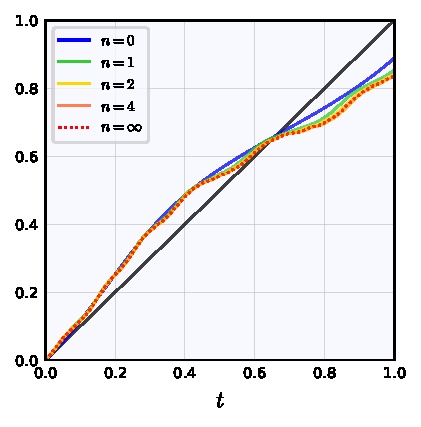
\includegraphics[height=0.48\linewidth]{figures/cont_dep1}
    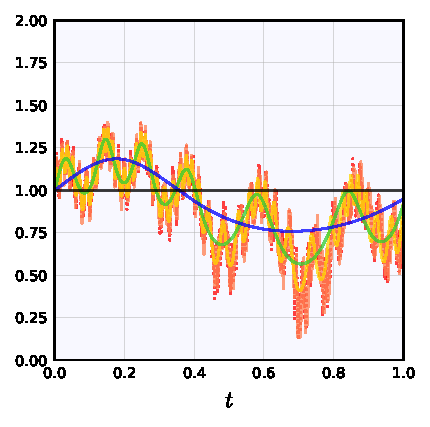
\includegraphics[height=0.48\linewidth]{figures/cont_dep2}
    \caption{The left panel shows the solutions $\vp_n$ of the IVPs $x'=f_n(t,x)$, $x(0)=0$ with $f_n$ as in \autoref{eq:cont_ex}. Also shown is the IVP solution when setting $w_n=0$ in \autoref{eq:cont_ex} (black). The right panel shows the corresponding volatility paths $\sqrt{\vp'_n}$.}
    \label{fig:cont_dependence}
\end{figure}

\subsection{Simulation of solutions}\label{sec:simulation}

The focus of this section is \autoref{thm:euler_converge}, which relates to a simple forward Euler simulation scheme for our IVPs $x'=f(t,x)$, $x(\tau)=\xi$ with $f\in\uF$. This result is not standard, however, since we never actually presume that values of this function $f$ can be reproduced \emph{exactly} on a computer, but just those of a \emph{convenient} sequence $\{f_n\}_{n\in\NN}\subset\uF$ converging uniformly (over compacts) to it. By convenient, we mean that (over compacts) each $f_n$ can be stored in computer memory. Beyond simple models, this generalised type of simulation convergence is often required in volatility modelling, and we will rely on it for applications in \autoref{chap:framework}.

Although computational ODE texts such as \cite{griffiths_2010} and \cite{han_2017} can be consulted for the Euler method and extensions, the related Cauchy-Peano existence theorem proof and its dependencies, e.g.~as in \cite{coddington_1955}, will prepare the reader better for \autoref{thm:euler_converge}. This is because we are not targeting a fancy simulation scheme of any sort, but for now a framework-wide one applicable for any $f\in\uF$, which is as simple as possible, notwithstanding the necessary generalisation just mentioned.

At first it can seem that \autoref{thm:euler_converge} here could follow from the continuous dependence result of \autoref{thm:continuity_solution_map}, or vice versa. But here, practicable polygons are being simulated which are not differentiable and can only be considered to solve IVPs driven by discontinuous functions, i.e.~in a Carath\'eordory sense. So \autoref{thm:continuity_solution_map}$\implies$\autoref{thm:euler_converge} would require an extension of \autoref{thm:continuity_solution_map} applicable to discontinuous functions such as $f_n\in\uD(\RR^2,\RR)$. This approach for obtaining \autoref{thm:euler_converge} is circumvented here through a simple application of Lebesgue's calculus to (absolutely continuous) polygons. In the other direction, we only get \autoref{thm:euler_converge}$\implies$\autoref{thm:continuity_solution_map} if in \autoref{thm:euler_converge} we take the mesh limit $\Vert\pi_n\Vert\to0$ \emph{before} taking $f_n\to f_0$. But such an iterated limit cannot actually be realised on a computer.

We now define an IVP's forward Euler polygon. Toward this, call an unbounded set $\pi:=\{t_k\}_{k\in\NN_0}\subset[\tau,\infty)$, with $\tau=:t_0<t_1<\dots$, a partition of $[\tau,\infty)$, and let $\Pi([\tau,\infty))$ be the set of such objects. For $T\in(\tau,\infty)$, define the mesh $\Vert\pi\Vert_{[\tau,T]}:=\max_{k\in\NN_0}\{t_{k+1}\wedge T - t_k\wedge T\}$. Finally, we write $\vp_\pi\in\uAC\subset\uC$ to emphasise \emph{absolute} continuity of the following polygons.

\begin{definition}[Forward Euler polygon]\label{alg:forward_euler}
    Fix $f\in\uC(\RR^2,\RR)$ and $\pi:=\{t_k\}_{k\in\NN_0}\in\Pi([\tau,\infty))$ for some $\tau\in\RR$, e.g.~one could set $t_k:=\tau+k\Delta$ for some $\Delta>0$. Define the polygon $\vp_\pi\in\uAC([\tau,\infty),\RR)$ using $\vp_\pi(\tau):=\xi\in\RR$, then recursively over each interval $(t_k,t_{k+1}]$ set
    \begin{equation}\label{alg:equation}
        \vp_\pi(t) := \vp_\pi(t_k) + (t-t_k) f(t_k,\vp_\pi(t_k))
    \end{equation}
    noticing that indeed $\vp_\pi(t)\xrightarrow{t\downarrow t_k}\vp_\pi(t_k)$ for every $k\in\NN_0$, and $\cup_{k\in\NN_0}(t_k,t_{k+1}]=(\tau,\infty)$. Such a path $\vp_\pi$ will be called the forward Euler $\pi$-polygon for the IVP $x'=f(t,x)$, $x(\tau)=\xi$.
\end{definition}

No harm comes from defining forward Euler polygons over all of $[\tau,\infty)$, even if maximal solutions $\vp\in\uC^1([\tau,T_*),\RR)$ of the related IVP $x'=f(t,x)$, $x(\tau)=\xi$ explode in finite time, e.g.~satisfy $T_*<X_*:=\lim_{t\uparrow T_*}\vp(t)=\infty$. Theoretically, our forward Euler polygons $\vp_\pi$ cannot explode over a compact $[\tau,T]$, as this would demand an infinitude of time points from $\pi$ to be in $[\tau,T]$. Practically, $\vp_\pi$ could of course exceed a computer's largest number.

We now give our convergence result on forward Euler polygons for \autoref{prob:ivp}. Its proof uses the modulus of continuity of a function $f\in\uF$ which, over compact $\cX\subset\RR^2$, is defined
\begin{equation}\label{eq:mod_cont_def}
    w(r) = w_{f,\cX}(r) := \sup\{|f(t_2,x_2)-f(t_1,x_1)|:|(t_2,x_2)-(t_1,x_1)|<r,(t_i,x_i)\in\cX\}.
\end{equation}
For any such $f$ and $\cX$, the existence of $w$ and the limit $w(r)\xrightarrow{r\downarrow0}0$ follow from $f\in\uC(\RR^2,\RR)$.

\begin{theorem}[Forward Euler convergence]\label{thm:euler_converge}
    Assume $\{f_n\}_{n\in\NN_0}\subset\uF$ and $f_n(\tau,\xi)>0$. For partitions $\{\pi_n\}_{n\in\NN}\subset\Pi([\tau,\infty))$, let $\vp_n\in\uAC([\tau,\infty),\RR)$ be the forward Euler $\pi_n$-polygon for the IVP $x'=f_n(t,x)$, $x(\tau)=\xi$, and let $\vp_0\in\uC^1([\tau,T_0),\RR)$ be the unique maximal solution of the IVP $x'=f_0(t,x)$, $x(\tau)=\xi$. Then for any values $T\in(\tau,T_0)$ and $X\in(\vp_0(T),\infty)$,
    \begin{equation}\label{eq:euler_converge}
        \left(\Vert f_0 - f_n \Vert_{[\tau,T]\times[\xi,X]}, \Vert\pi_n\Vert_{[\tau,T]}\right) \xrightarrow{n\to\infty}(0,0) \implies \Vert\vp_0 - \vp_n\Vert_{[\tau,T]}\xrightarrow{n\to\infty}0.
    \end{equation}
\end{theorem}
\begin{proof}
    Unlike the IVP solutions from \autoref{thm:continuity_solution_map}, a given polygon $\vp_n$ need not be strictly increasing like $\vp_0$, and indeed the bounds from \autoref{lem:spatial_bounds} may be violated, e.g.~we could find $\vp_n(t)<\xi$ for some $n$ and $t>\tau$. Nevertheless, as with \autoref{thm:continuity_solution_map}, fix $T\in(\tau,T_0)$ and $X\in(\vp_0(T),X_0)$, then define the rectangle $\cX:=[\tau,T]\times[\xi,X]$. We will now clarify that, over some subinterval $[\tau,t_1]\subset[\tau,T]$, we still find $(t,\vp(t))\in\cX$ for sufficiently large $n$.

    Since $f_0(\tau,\xi)>0$ and $f_0(\cdot,\xi)$ is strictly increasing, then $f_0(t,\xi)>0$ over $[\tau,T]$, and the continuity of $f_0$ provides a rectangle $\cX_\ep:=[\tau,T]\times[\xi,\xi+\ep]\subset\cX$ where $f_0(t,x)>0$ also. Using $\Vert f_0 - f_n \Vert_{\cX_\ep}\xrightarrow{n\to\infty}0$, this can be extended w.l.o.g.~to every $n$, i.e.~we can assume $f_n(t,x)>0$ for all $n$ provided $(t,x)\in\cX_\ep$. Precisely as in \autoref{thm:continuity_solution_map}, the wider convergence $\Vert f_0 - f_n \Vert_\cX \xrightarrow{n\to\infty}0$ also allows us to assume w.l.o.g.~a bound $\Vert f_n \Vert_\cX<M$ for all $n$.

    The rectangular sliver $\cX_\ep$ will become a reflecting barrier for the polygons $\vp_n$ for sufficiently large $n$, reestablishing the bound $\vp_n(t)\ge\xi$ as $n\to\infty$. To see this, consider $\vp_n$ over $[\tau,t_1]$ where $t_1:=\tau+M^{-1}(X-\vp_0(T))$ as in \autoref{thm:continuity_solution_map}. Since $\Vert f_n \Vert_\cX<M$, $\vp_n$ cannot reach the top of $\cX$ over $[\tau,t_1]$, but it could reach the bottom. To pull this off, however, $\vp_n$ must first escape through the top of $\cX_\ep$, to find a point where $f_n(t,x)<0$. For $\vp_n$ to \emph{then} reach the bottom of $\cX$ requires the crossing of $\cX_\ep$ in one forward Euler step, since $f_n(t,x)>0$ in $\cX_\ep$. This becomes impossible once the simulation mesh is sufficiently small, specifically once $\Vert\pi_n\Vert_{[\tau,t_1]}<M^{-1}\ep$. Since this is guaranteed by assumption as $n\to\infty$, we can now assume w.l.o.g.~that it holds for all $n$ so that, over $[\tau,t_1]$ at least, all $\vp_n$ are now contained in $\cX$.

    Now getting $\Vert \vp_0 - \vp_n\Vert_{[\tau,t_1]} \xrightarrow{n\to\infty}0$ utilises the general approach in \autoref{eq:approach_summary}, but the details are a little different to those of \autoref{thm:continuity_solution_map}, since $\vp_n(t)\neq \xi + \int_\tau^t f_n(s,\vp_n(s))\dd s$, i.e.~$\vp_n$ is not an IVP solution but rather a forward Euler polygon. Given however $\vp_n\in\uAC([\tau,\infty),\RR)$, then we at least have $\vp_n(t) = \xi + \int_{[\tau,t]} \vp'_n(s)\dd s$, which can be written
    \begin{equation}\label{eq:main_sim}
        \vp_n(t) = \xi + \int_{[\tau,t]} f_0(s,\vp_n(s)) + \lambda_n(s)\dd s,\quad \lambda_n(t) := \vp'_n(t) - f_0(t,\vp_n(t)).
    \end{equation}
    Notice the subtle difference between $\lambda_n$ here and in \autoref{eq:cont_dep_main}. For each $t\in[\tau,T]$, let $t_n=t_n(t):=\max\{t_k\in\pi_n:t_k<t\}$ denote the time point in the partition $\pi_n$ which immediately precedes $t$, so that $0<t-t_n\le \Vert\pi_{n}\Vert_{[\tau,T]}$ and $\vp'_n(t)=f_n(t_n,\vp_n(t_n))$ wherever $\vp'_n$ exists. Substituting this equality into $\lambda_n$ from \autoref{eq:main_sim}, for a.e.~$t\in[\tau,t_1]$ we obtain
    \begin{multline}\label{eq:lambda_bound}
        |\lambda_n(t)| = |f_n(t_n,\vp_n(t_n)) - f_0(t,\vp_n(t))|\\
        \le\underbrace{|f_n(t_n,\vp_n(t_n)) - f_0(t_n,\vp_n(t_n))|}_{\le \Vert f_n-f_0\Vert_\cX\xrightarrow{n\to\infty}0} + \underbrace{|f_0(t_n,\vp_n(t_n)) - f_0(t,\vp_n(t)) |}_{\le w(\sqrt{1+M^2}\Vert\pi_{n}\Vert_{[\tau,T]})\xrightarrow{n\to\infty}0}
    \end{multline}
    which utilises the triangle inequality, the bound $|(t_n,\vp_n(t_n)) - (t,\vp_n(t)) |<\sqrt{1+M^2}\Vert\pi_{n}\Vert_{[\tau,T]}$, and the modulus of continuity $w=w_{f_0,\cX}$ from \autoref{eq:mod_cont_def}, which satisfies $w(r)\xrightarrow{r\downarrow0}0$.

    Having ensured $\Vert\vp_n\Vert_{[\tau,t_1]}<|\xi|\vee|X|$ and $\Vert\vp'_n\Vert_{[\tau,t_1]}<M$, the set $\{\vp_n\}_{n\in\NN_0}$ is equibounded and equicontinuous over $[\tau,t_1]$. Like in the proof of \autoref{thm:continuity_solution_map}, assuming the limit $\Vert\vp_0 - \vp_n\Vert_{[\tau,t_1]}\xrightarrow{n\to\infty}0$ is violated leads to a contradiction, by invoking the Ascoli Lemma and the limit $\int_{[\tau,t]} \lambda_n(s)\dd s\xrightarrow{n\to\infty}0$ in \autoref{eq:main_sim} to get a limit $\vp_*:=\lim_{k\to\infty}\vp_{n_k}\neq\vp_0$ which verifies $\vp_*(t)= \xi + \int_\tau^t f_0(s,\vp_*(s))\dd s$ like $\vp_0$. So we must conclude $\Vert\vp_n-\vp_0\Vert_{[\tau,t_1]}\xrightarrow{n\to\infty}0$, and again as in \autoref{thm:continuity_solution_map}, this can be extended in steps to any $[\tau,t_k\wedge T]$ with $t_k:=\tau + kM^{-1}(X-\vp_0(T))$, providing the claim of $\Vert\vp_n-\vp_0\Vert_{[\tau,T]}\xrightarrow{n\to\infty}0$ after $\lceil\frac{T-\tau}{t_1-\tau}\rceil$ steps.
\end{proof}

Given the generality of the partitions $\{\pi_n\}_{n\in\NN}\subset\Pi([\tau,\infty))$ in \autoref{thm:euler_converge}, we are free to decouple the assumption in \autoref{eq:euler_converge} to $\lim_{(n,m)\to(\infty,\infty)}\left(\Vert f_0 - f_n \Vert, \Vert\pi_m\Vert\right)$ $=(0,0)$. By utilising \autoref{thm:euler_converge} as stated and \autoref{thm:continuity_solution_map} from the previous section, it is then straightforward to establish that this joint limit can be replaced with either iterated variant $\lim_{n\to\infty}\lim_{m\to\infty}$ or $\lim_{m\to\infty}\lim_{n\to\infty}$. As already discussed, however, such iterated limits cannot be realised on a computer and so by themselves are not actually practically useful.

\vspace{4mm}To illustrate \autoref{thm:euler_converge}, in \autoref{fig:sim_converge1} we reproduce \autoref{fig:main_examples} but also show sequences of forward Euler polygons $\vp_n$ converging to the IVP solution $\vp_0$. Dyadic and triadic partitions are used, defined by $\pi_n:=\{k m^{-n}:k\in\NN_0\}$ for $m=2,3$ respectively. For simplicity, $f_n:=f$ for all $n$, where $f(t,x):=\sigma w(x)+\kappa(\theta t - x)+v$ is the Heston function from \autoref{fig:weierstrass_example}.

\begin{figure}[H]
    \centering
    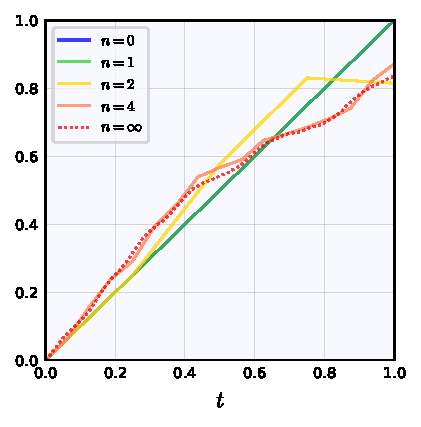
\includegraphics[height=0.48\linewidth]{figures/sim1}
    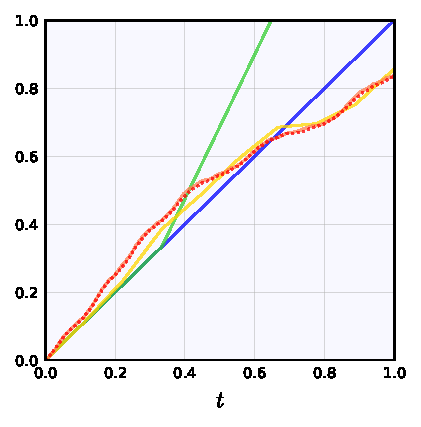
\includegraphics[height=0.48\linewidth]{figures/sim2}
    \caption{The left panel shows forward Euler polygons converging to the IVP solution from \autoref{fig:main_examples} when using dyadic partitions. The right panel repeats the left but uses instead triadic partitions, so converges faster.}
    \label{fig:sim_converge1}
\end{figure}

\vspace*{-4mm}
In general, we cannot bound the rates of convergence illustrated in \autoref{fig:sim_converge1} without imposing constraints on the spatial regularity of $f(t,x):=\sigma w(x)+\kappa(\theta t - x)+v$ via $w$. Nevertheless when we come to draw comparisons between our new volatility models and existing ones in \autoref{sec:vol_surfaces}, it is still important to gauge the error imparted by our forward Euler scheme on the metrics being compared. In \autoref{fig:heston_comparison_skewed} and \autoref{fig:heston_comparison_symmetric} the metrics being compared are implied volatilities, and we find that 4,096 simulated paths are sufficient to bring all simulated implied volatilities within 0.1 of the analytically generated Heston ones. Each one of these 4,096 paths depends on our forward Euler scheme from \autoref{alg:forward_euler}, and in the \hyperlink{appendix}{Appendix} we provide succinct \texttt{python} code which generates one such path with 4,096 time steps over 10 years, i.e.~using $\Delta:=10/4,096\approx0.0024$ in \autoref{alg:forward_euler}. As explained in the \hyperlink{appendix}{Appendix}, this code takes 75 ms to run on a 2.3 GHz Intel Core i5 MacBook Pro.

This concludes the present chapter, so the treatment of well-posedness for \autoref{prob:ivp}. While it is tempting to include here some minor modifications of this problem, especially regarding the delicate possibility of relaxing the assumption of $f(\tau,\xi)>0$ to $f(\tau,\xi)\ge0$, this seems better placed in the next chapter, which explores the solution space and its limits.
